\documentclass[12pt,a4paper,oneside]{report}

% ---------------------------------------------------------------- fonts and layout (Amrita report format)
\usepackage{fontspec}
\setmainfont{TeX Gyre Termes}
\usepackage{amsmath,amssymb}
\usepackage[a4paper,top=30mm,bottom=28mm,left=25mm,right=22mm,headheight=15pt]{geometry}
\usepackage{setspace}
\setstretch{1.25}
\usepackage{graphicx}
\usepackage{booktabs,tabularx,longtable,array}
\usepackage{float}
\usepackage[labelfont=bf,font=small]{caption}
\usepackage{enumitem}
\setlist{itemsep=2pt,topsep=4pt}
\usepackage{xcolor}
\usepackage{titlesec}
\usepackage{tocloft}
\usepackage{fancyhdr}
\usepackage[hidelinks]{hyperref}
\usepackage{microtype}

\graphicspath{{figs/}}
\emergencystretch=3em
\newcolumntype{L}[1]{>{\raggedright\arraybackslash}p{#1}}
\newcolumntype{Y}{>{\raggedright\arraybackslash}X}
\renewcommand{\arraystretch}{1.15}

% chapter heading: "Chapter N" then the title, both bold, left aligned
\titleformat{\chapter}[display]{\normalfont\LARGE\bfseries}{\chaptertitlename\ \thechapter}{18pt}{\LARGE}
\titlespacing*{\chapter}{0pt}{10pt}{24pt}
\titleformat{\section}{\normalfont\Large\bfseries}{\thesection}{1em}{}
\titleformat{\subsection}{\normalfont\large\bfseries}{\thesubsection}{1em}{}

% running head "CHAPTER N. TITLE" with a rule, page number at the bottom centre
\pagestyle{fancy}
\fancyhf{}
\renewcommand{\chaptermark}[1]{\markboth{\MakeUppercase{\chaptername\ \thechapter.\ #1}}{}}
\fancyhead[R]{\small\leftmark}
\fancyfoot[C]{\thepage}
\renewcommand{\headrulewidth}{0.4pt}
\fancypagestyle{plain}{\fancyhf{}\fancyfoot[C]{\thepage}\renewcommand{\headrulewidth}{0pt}}

% contents with dotted leaders, bold chapter entries
\renewcommand{\cftchapleader}{\hfill}
\setlength{\cftbeforechapskip}{10pt}
\renewcommand{\contentsname}{Contents}
\renewcommand{\cftloftitlefont}{\LARGE\bfseries}
\renewcommand{\cftlottitlefont}{\LARGE\bfseries}
\renewcommand{\cfttoctitlefont}{\LARGE\bfseries}

\newcommand{\ra}{$\rightarrow$}
\newcommand{\COtwo}{CO\textsubscript{2}}
\newcommand{\frontheading}[1]{\chapter*{#1}\addcontentsline{toc}{chapter}{#1}}

\newcommand{\reporttitle}{Smart Classroom Energy Management: Occupancy-Driven Lighting and Air-Conditioning Control using IoT and Machine Learning}

\begin{document}

% ================================================================ TITLE PAGE
\begin{titlepage}
\newgeometry{top=18mm,bottom=16mm,left=22mm,right=22mm}
\centering
\setstretch{1.1}
{\LARGE\bfseries AMRITA SCHOOL OF COMPUTING\par}
\vspace{1mm}
{\large AMRITA VISHWA VIDYAPEETHAM\par}
{\large AMRITAPURI\par}
\vspace{5mm}

\includegraphics[width=30mm]{amrita_logo.jpg}\par
\vspace{8mm}
{\Large\bfseries Smart Classroom Energy Management:\\ Occupancy-Driven Lighting and Air-Conditioning\\ Control using IoT and Machine Learning\par}
\vspace{7mm}
{\normalsize Report submitted for\par}
\vspace{1mm}
{\large\bfseries INTERNET OF THINGS PROJECT REPORT\par}
\vspace{7mm}
{\normalsize submitted by\par}
\vspace{2mm}
{\normalsize
\begin{tabular}{ll}
NIRANJAN N S & AM.SC.U4CSE23338\\
SIVADEV SMIJITH & AM.SC.U4CSE23359\\
YALAMARTHI JYOTHI SRI KRISHNA CHAITANYA & AM.SC.U4CSE23370\\
PENUMALLU RAM DINESH REDDY & AM.SC.U4CSE23341\\
MANISH SHISHIRCHANDRA DORA ALURI & AM.SC.U4CSE23333\\
\end{tabular}\par}
\vspace{7mm}
{\normalsize under the guidance of\par}
\vspace{2mm}
{\large Dr. Sangeeth Kumar\par}
{\normalsize Associate Professor\par}
{\normalsize Center for Wireless Networks \& Applications (Amrita WNA)\par}
\vspace{8mm}
{\normalsize Amrita School of Computing\par Amrita Vishwa Vidyapeetham\par Amritapuri\par}
\vspace{4mm}
{\normalsize Academic Year: 2026--2027\par}
\end{titlepage}
\restoregeometry

% blank page after the title page, as in the department format
\thispagestyle{empty}\null\clearpage

\pagenumbering{roman}
\setcounter{page}{2}
\pagestyle{plain}

% ================================================================ CERTIFICATE
\chapter*{Certificate}
\addcontentsline{toc}{chapter}{Certificate}
This is to certify that the project report titled \textbf{``\reporttitle''} is a bona fide record of the work carried
out by the following students under my guidance, in partial fulfilment of the requirements for the Internet of Things
project component of the B.Tech programme, Department of Computer Science and Engineering, Amrita School of
Computing, Amrita Vishwa Vidyapeetham, Amritapuri, during the academic year 2026--2027.

\vspace{6mm}
\begin{center}
\begin{tabular}{ll}
\toprule
\textbf{Name} & \textbf{Roll Number}\\
\midrule
NIRANJAN N S & AM.SC.U4CSE23338\\
SIVADEV SMIJITH & AM.SC.U4CSE23359\\
YALAMARTHI JYOTHI SRI KRISHNA CHAITANYA & AM.SC.U4CSE23370\\
PENUMALLU RAM DINESH REDDY & AM.SC.U4CSE23341\\
MANISH SHISHIRCHANDRA DORA ALURI & AM.SC.U4CSE23333\\
\bottomrule
\end{tabular}
\end{center}

\vspace{18mm}
\noindent
\begin{minipage}[t]{0.52\textwidth}
Dr. Sangeeth Kumar\\
Associate Professor\\
Center for Wireless Networks \&\\ Applications (Amrita WNA)\\
Amritapuri
\end{minipage}\hfill
\begin{minipage}[t]{0.44\textwidth}
Dr. Lekha S Nair\\
Head of the Department\\
Department of Computer Science and Engineering
\end{minipage}

\vspace{14mm}
\noindent Place: Amritapuri\\
Date: 04/11/2026

% ================================================================ DECLARATION
\chapter*{Declaration}
\addcontentsline{toc}{chapter}{Declaration}
We hereby declare that the project report titled \textbf{``\reporttitle''} is an original record of work carried out
by us under the guidance of \textbf{Dr. Sangeeth Kumar}, Associate Professor, Center for Wireless Networks \&
Applications (Amrita WNA), Amrita Vishwa Vidyapeetham, Amritapuri, and that it has not been submitted elsewhere for
the award of any degree or diploma. All measured data analysed in this report come from the public ROBOD dataset
(Tekler et al., 2022). Every predicted value comes from our models, and every simulated value (actuator states,
controlled energy, room simulation) is labelled as simulated. No result has been fabricated, and wherever something
could not be verified the report says so.

\vspace{14mm}
\noindent
\begin{tabular}{@{}ll}
NIRANJAN N S & AM.SC.U4CSE23338\\
SIVADEV SMIJITH & AM.SC.U4CSE23359\\
YALAMARTHI JYOTHI SRI KRISHNA CHAITANYA & AM.SC.U4CSE23370\\
PENUMALLU RAM DINESH REDDY & AM.SC.U4CSE23341\\
MANISH SHISHIRCHANDRA DORA ALURI & AM.SC.U4CSE23333\\
\end{tabular}

\vspace{10mm}
\noindent Place: Amritapuri\\
Date: 04/11/2026

% ================================================================ ACKNOWLEDGEMENT
\chapter*{Acknowledgement}
\addcontentsline{toc}{chapter}{Acknowledgement}
We are sincerely grateful to \textbf{Dr. Sangeeth Kumar}, Associate Professor, Center for Wireless Networks \&
Applications (Amrita WNA), Amrita Vishwa Vidyapeetham, Amritapuri, for his steady guidance, constructive feedback and
support throughout this project.

Our thanks also go to the faculty and staff of the Department of Computer Science and Engineering, Amrita Vishwa
Vidyapeetham, Amritapuri, for their support while the project was under way.

We acknowledge the authors of the ROBOD dataset (Tekler, Lei, Peng, Miller and Chong), whose openly published
lecture-room data made this work possible. We also acknowledge the open-source communities behind Eclipse
Mosquitto, Node-RED, SQLite, scikit-learn and PyTorch.

Finally, we thank our families and friends for their encouragement.

\vspace{10mm}
\noindent NIRANJAN N S\\
SIVADEV SMIJITH\\
YALAMARTHI JYOTHI SRI KRISHNA CHAITANYA\\
PENUMALLU RAM DINESH REDDY\\
MANISH SHISHIRCHANDRA DORA ALURI

% ================================================================ ABSTRACT
\chapter*{Abstract}
\addcontentsline{toc}{chapter}{Abstract}
This project builds an end-to-end Internet of Things system that monitors lecture rooms and controls their lighting
and air-conditioning (AC) from occupancy analytics. It follows the eight-stage reference architecture:

\begin{itemize}
\item an IoT node replays the real ROBOD dataset (two lecture rooms, 5-minute data, 29 weekdays) to an
  authenticated Mosquitto MQTT broker;
\item Node-RED validates, stores (SQLite), visualises (Node-RED Dashboard 2.0) and decides;
\item a Python service runs traditional, ensemble and deep-learning occupancy models;
\item simulated light and AC actuators on a second laptop execute the commands and acknowledge them.
\end{itemize}

Two recent research methods are integrated as adaptations: a Mamba selective state-space occupancy model (the model
family of OCC-Mamba) and an LSTM + Dueling Deep Q-Network HVAC controller (Hou et al., 2025).

\textbf{Model results.} On six held-out test dates, Mamba reached the best test F1 (0.651). The random forest, selected
by validation F1 before the test dates were scored, reached 0.559. A date-cluster bootstrap shows that the models are
not significantly different on this amount of data.

\textbf{Energy results} (all simulated):
\begin{itemize}
\item Rule-based control with predicted occupancy used 52\% less simulated cooling than always-on operation (405.5 vs
  850.6~kWh thermal over six test days), with 0.6\% of occupied intervals outside the comfort band.
\item On recorded energy re-scaled by our commands, it saved 38.7\% of lighting and 39.5\% of chilled-water energy,
  but switched the lights off in 27.9\% of occupied intervals. This comfort cost is reported alongside every saving.
\item The Dueling DQN saves more energy but violates comfort more often, so rules remain the default.
\end{itemize}

\textbf{Engineering results.} The live loop acknowledged 100\% of commands, with a median round trip of 88~ms. The
project has 97 automated tests and an end-to-end test, all passing.

\vspace{4mm}
\noindent\textbf{Keywords:} Internet of Things, MQTT, Node-RED, occupancy estimation, smart building, energy
management, Mamba, Dueling DQN.

% ================================================================ CONTENTS, LISTS
\tableofcontents
\clearpage
\listoffigures
\clearpage
\listoftables
\clearpage

\chapter*{List of Abbreviations}
\addcontentsline{toc}{chapter}{List of Abbreviations}
\begin{longtable}{@{}L{3.2cm}L{11.5cm}@{}}
\toprule
\textbf{Abbreviation} & \textbf{Expansion}\\
\midrule
\endhead
ACL & Access Control List (MQTT broker topic permissions)\\
AC & Air-Conditioning\\
ACK & Acknowledgement (actuator feedback message)\\
BMS & Building Management System\\
CI & Confidence Interval\\
\COtwo{} & Carbon dioxide (indoor air-quality indicator)\\
CV & Cross-Validation\\
DQN & Deep Q-Network\\
ECO & Energy-saving AC mode (raised set-point)\\
F1 & Harmonic mean of precision and recall\\
FCU & Fan Coil Unit\\
HVAC & Heating, Ventilation and Air-Conditioning\\
IAQ & Indoor Air Quality\\
IoT & Internet of Things\\
K$\cdot$h & Kelvin-hours (comfort violation magnitude)\\
LAN & Local Area Network\\
LSTM & Long Short-Term Memory network\\
LWT & Last Will and Testament (MQTT)\\
MAE & Mean Absolute Error\\
ML & Machine Learning\\
MQTT & Message Queuing Telemetry Transport\\
QoS & Quality of Service (MQTT delivery guarantee)\\
RC & Resistance--Capacitance (thermal model)\\
RF & Random Forest\\
RMSE & Root Mean Squared Error\\
ROBOD & Room-level Occupancy and Building Operation Dataset\\
RTT & Round-Trip Time\\
SSM & State-Space Model\\
TLS & Transport Layer Security\\
{[M] / [P] / [S]} & Measured / Predicted / Simulated value (labels used throughout)\\
\bottomrule
\end{longtable}

% ================================================================ MAIN MATTER
\clearpage
\pagenumbering{arabic}
\setcounter{page}{1}
\pagestyle{fancy}

% ---------------------------------------------------------------- Chapter 1
\chapter{Introduction}

\section{Background}
Lighting and air-conditioning are among the largest energy loads in teaching buildings, and they often run while
rooms are empty: between lectures, after the last class, during cancelled sessions. In warm, humid climates the
chilled water that cools a lecture room is the dominant load. In the six Room~1 test days of the ROBOD dataset, the
room recorded 923~kWh of chilled-water thermal energy and 85.6~kWh of lighting electrical energy, while about 80\% of
its 5-minute intervals were empty according to the camera ground truth.

The Internet of Things (IoT) makes it possible to sense a room, reason about its occupancy and act on the result
automatically. A practical system needs more than a model, though. It needs reliable messaging, integration,
storage, visualisation, a safe decision layer, and confirmation that each command was actually executed. This
project builds such a system on the reference architecture prescribed by the faculty, using real lecture-room data.

\section{Problem Statement}
The faculty problem statement for Team~1 asks for a system that:
\begin{itemize}
\item \textbf{monitors} occupancy, temperature, ambient light and electrical power;
\item \textbf{estimates} occupied and unoccupied periods and energy demand with analytical or machine-learning
  methods;
\item \textbf{controls} lighting and AC from those analytics, reducing energy in expected unoccupied periods and/or
  preparing the room before expected occupancy.
\end{itemize}

The architecture is prescribed: an IoT node (real data or simulator), MQTT, Node-RED for integration and automation,
SQLite or MySQL, and the Node-RED Dashboard.

\section{Objectives}
\begin{enumerate}
\item \textbf{O1:} implement all eight reference stages, split across a server laptop and an IoT-node laptop.
\item \textbf{O2:} compare traditional, ensemble and deep-learning models fairly, on predictive, computational and
  closed-loop performance.
\item \textbf{O3:} integrate two 2024--2026 research algorithms, and state honestly what was adapted.
\item \textbf{O4:} control both loads safely, with complete command and acknowledgement feedback.
\item \textbf{O5:} report energy and comfort honestly, separating measured, predicted and simulated quantities.
\item \textbf{O6:} make the system testable, reproducible, reasonably secure on a LAN, and demonstrable live.
\end{enumerate}

\section{Scope}
\textbf{In scope:}
\begin{itemize}
\item two ROBOD lecture rooms replayed as the IoT node;
\item occupancy now (presence), next-5-minute energy, and arrival within 30 minutes (pre-cooling);
\item lighting (ON/DIM/OFF) and AC (OFF/ECO/COMFORT/BOOST/PRECOOL) control through simulated actuators;
\item energy and comfort evaluation in a recorded-energy counterfactual and in a grey-box room simulator.
\end{itemize}

\textbf{Out of scope:} real relays or BMS integration, metered real-world savings, camera-based people counting,
multi-building deployment, TLS certificate management and cloud hosting.

\section{Significance of the Study}
The project puts a complete IoT control loop to work on real building data, and holds itself to one rule on
integrity: every number in this report is traceable to a result file produced by the project's own scripts. Every
saving is labelled as simulated. Test data was never used for training, model selection or threshold tuning. The
same code that runs live is executed by the automated tests and the experiments, so the reported behaviour is the
deployed behaviour.

\section{Methodology Overview}
\begin{enumerate}
\item The ROBOD data were verified (SHA-256, schema) and split by whole date into training, validation and test
  dates.
\item Leak-free features were built.
\item Seven occupancy models (including a baseline and the two research models) were trained and compared, together
  with an energy forecaster and an arrival profile.
\item A Dueling DQN was trained in a grey-box room simulator.
\item The decision engine was implemented once, in Node-RED, and evaluated in closed loop.
\item The full system was run live over MQTT and checked by 97 automated tests and an end-to-end test.
\end{enumerate}

\section{Organisation of the Report}
\begin{itemize}
\item Chapter~\ref{ch:lit} reviews the dataset and the two research papers.
\item Chapter~\ref{ch:req} sets out the requirements, hardware and software, and the constraints.
\item Chapter~\ref{ch:design} describes the system design and methods, from MQTT to the Dueling DQN.
\item Chapter~\ref{ch:results} presents the results: model evaluation, energy and comfort, performance, testing and
  deployment.
\item Chapter~\ref{ch:concl} concludes with limitations, future work and team contributions.
\item The appendix gives the reproduction instructions.
\end{itemize}

% ---------------------------------------------------------------- Chapter 2
\chapter{Literature Review}\label{ch:lit}

\section{ROBOD Dataset}
ROBOD (Tekler, Lei, Peng, Miller and Chong, 2022) provides room-level occupancy and building operation data for
lecture rooms, offices and a library at the National University of Singapore. It includes Wi-Fi connected devices,
\COtwo{}, sound, humidity, temperature and illuminance; plug, lighting, fan and chilled-water energy; and
camera-derived occupancy labels. The camera labels make supervised occupancy estimation possible and give an oracle
upper bound for control experiments.

\section{Paper A: OCC-Mamba}
I.~Qaisar, K.~Sun, D.~Zhong, X.~Yang, X.~Miao and Q.~Zhao, \emph{OCC-Mamba: A Mamba-based deep learning approach for
indoor occupancy prediction}, Building and Environment, article 114085 (2025).

We verified the bibliographic record. We could \textbf{not} access the abstract, full text or code: the publisher
blocks automated access and no repository is listed. Our implementation therefore follows the \textbf{Mamba
mechanism} (Gu and Dao, 2023). In Mamba, the state-space step size $\Delta$ and the matrices $B$ and $C$ depend on the
input, so the recurrence can keep or forget information at each time step, and it runs in linear time. We do not
claim OCC-Mamba's configuration, inputs or results.

\section{Paper B: LSTM and Dueling DQN}
F.~Hou, J.~C.~P.~Cheng, J.~Ma, H.~H.~L.~Kwok, C.~Huang and Z.~Wu, \emph{Occupancy-driven HVAC control optimization
via LSTM and deep reinforcement learning for enhanced indoor air quality, thermal comfort and energy efficiency},
Building and Environment 284 (2025) 113501.

\textbf{Method (from the published abstract).} An LSTM estimates occupancy from indoor \COtwo{} fluctuations, using
labels derived by change-point analysis. A Dueling DQN (Wang et al., 2016) then reduces HVAC operation in unoccupied
periods while maintaining thermal comfort and indoor air quality.

\textbf{Reported results (theirs, not ours).}
\begin{itemize}
\item about 0.7 precision and 0.6 recall for occupancy estimation;
\item 9.5--14.6\% fewer temperature violations;
\item 10.9--30.4\% less HVAC operation time.
\end{itemize}
The exact state, action and reward definitions were not accessible to us.

\section{Gaps and Need for the Study}
The two papers are complementary. A is a modern sequence model for the prediction stage. B closes the loop from
prediction to HVAC action. Neither describes a complete, reproducible IoT deployment on the prescribed architecture
with delivery-confirmed actuation, and neither reports savings next to the comfort cost of wrong decisions in a way
that can be checked from public data. This project integrates both methods into such a system, compares them with
traditional and ensemble baselines on held-out dates, and reports every saving with its comfort cost.

\begin{table}[H]
\centering
\caption{Summary of reviewed literature and relevance to the present study}
\label{tab:lit}
\begin{tabularx}{\textwidth}{@{}L{3.6cm}YY@{}}
\toprule
\textbf{Work} & \textbf{Contribution} & \textbf{Use in this project}\\
\midrule
Tekler et al. (2022), ROBOD & lecture-room sensor, energy and camera-occupancy dataset & the IoT node's data and the ground truth\\
Qaisar et al. (2025), OCC-Mamba & Mamba-based occupancy prediction & model family of our deep-learning model A\\
Gu and Dao (2023), Mamba & selective state-space sequence model & the mechanism we implemented\\
Hou et al. (2025) & LSTM occupancy + Dueling DQN HVAC control & our LSTM and Dueling DQN controller (B)\\
Wang et al. (2016) & dueling network architecture & the Q-network head\\
\bottomrule
\end{tabularx}
\end{table}

% ---------------------------------------------------------------- Chapter 3
\chapter{Problem Definition and Requirements}\label{ch:req}

\section{Detailed Problem Description}
The system must decide, every five minutes and for each room, whether the room is occupied, and set lighting and AC
accordingly. It must do this on the prescribed architecture, over a network between two laptops. Commands must be
confirmed, and failures (a lost broker, a missing model, a stale sensor) must be handled safely. Energy savings must
be weighed against comfort, because a controller that saves energy by switching off occupied rooms does not solve
the problem.

\section{Project Requirements}
\subsection{Functional Requirements}
\begin{itemize}
\item Replay real sensor data as an IoT node over MQTT; validate, store and visualise every reading.
\item Predict occupancy with several model families; forecast energy; estimate arrivals for pre-cooling.
\item Decide lighting and AC commands; send them over MQTT; receive and record acknowledgements.
\item Provide manual override, alerts for invalid or stale data, and device-health monitoring.
\end{itemize}
\subsection{Analytical Requirements}
\begin{itemize}
\item Use whole-date splits, so that test dates are never used for training, selection or tuning.
\item Compare against baselines, and report predictive, computational and closed-loop metrics.
\item Separate measured, predicted and simulated values everywhere.
\end{itemize}

\section{Hardware and Software Requirements}
\begin{table}[H]
\centering
\caption{Hardware and software requirements}
\label{tab:hwsw}
\begin{tabularx}{\textwidth}{@{}L{3.0cm}YL{3.6cm}@{}}
\toprule
\textbf{Item} & \textbf{Laptop 1 (server)} & \textbf{Laptop 2 (node)}\\
\midrule
OS & Windows 10/11 (Linux/macOS scripts also provided) & Windows 10/11\\
CPU / RAM / disk & any x86-64, 8~GB RAM, about 3~GB disk & 4~GB RAM, about 300~MB\\
Python & 3.11--3.13 (developed and tested on 3.13) & same\\
Node.js & 22 LTS ($\geq$ 20.17); tested on 22.23.4 & --\\
Mosquitto & 2.x (tested 2.0.18) & --\\
Python packages (pinned) & numpy 2.2.6, pandas 2.2.3, paho-mqtt 2.1.0, scikit-learn 1.6.1, scipy 1.15.3, joblib 1.4.2, torch 2.14.1, psutil 7.1.3, matplotlib 3.10.7, pytest 8.4.2 & numpy, pandas, paho-mqtt only\\
Node packages (pinned) & node-red 4.1.17, @flowfuse/node-red-dashboard 1.34.0, node-red-node-sqlite 2.0.1 & --\\
Network & same private LAN or hotspot; TCP 1883 and 1880 open on the Private profile, local subnet only & --\\
\bottomrule
\end{tabularx}
\end{table}

\section{Constraints and Assumptions}
\begin{itemize}
\item ROBOD contains no light or AC states, so all actuator states are simulated.
\item ROBOD cannot identify the room's thermal plant (linear models explained $R^2 \leq 0.044$ of temperature
  change), so closed-loop experiments use a grey-box simulator with declared, assumed parameters.
\item The dataset licence could not be verified, so the CSV files are downloaded from the official repository and
  checked against their SHA-256 values, never redistributed.
\item The full text of OCC-Mamba was not accessible; paper B's exact state, action and reward definitions were not
  accessible either.
\item The system is a LAN prototype: authenticated MQTT with an ACL, but no TLS.
\end{itemize}

% ---------------------------------------------------------------- Chapter 4
\chapter{System Design and Methods}\label{ch:design}

\section{Dataset Description}
\begin{table}[H]
\centering
\caption{ROBOD dataset as used in this project}
\label{tab:data}
\begin{tabularx}{\textwidth}{@{}L{3.0cm}Y@{}}
\toprule
\textbf{Property} & \textbf{Value}\\
\midrule
Rooms & Room 1 (primary: training, validation, test); Room 2 (cross-room evaluation only)\\
Size & 8,352 rows $\times$ 28 columns per room; 5-minute resolution\\
Period & 29 weekdays: 7 Sep--1 Oct and 9--23 Dec 2021; timestamps kept in +08:00\\
Integrity & SHA-256 Room 1 \texttt{34a3d7a1\ldots3f3d}, Room 2 \texttt{ac9a34cd\ldots941f}; checked by \texttt{download\_data.py} with schema (18 required columns) and row count\\
Licence & unverified; CSVs not redistributed\\
Missing data & Room 1: 14 rows without indoor sensors, 10 without chilled-water/fan energy; Room 2: 30 rows\\
\bottomrule
\end{tabularx}
\end{table}

\textbf{Units.} Lighting, FCU fan and plug energy are \textbf{electrical} kWh per 5 minutes. Chilled-water energy is
\textbf{thermal} kWh per 5 minutes and is never added to electrical energy.

\textbf{Splits (seed 42, by whole date):}
\begin{itemize}
\item 19 training dates;
\item 4 validation dates (2021-09-08, 09-27, 12-09, 12-13), used for model selection, early stopping and threshold
  tuning;
\item 6 test dates (2021-09-20, 09-21, 09-24, 09-30, 12-15, 12-22), used for reporting only.
\end{itemize}
That gives 5,414 / 1,119 / 1,717 usable rows. Two test dates are almost empty (0 and 1 occupied intervals).

\section{System Architecture}
\begin{figure}[H]
\centering
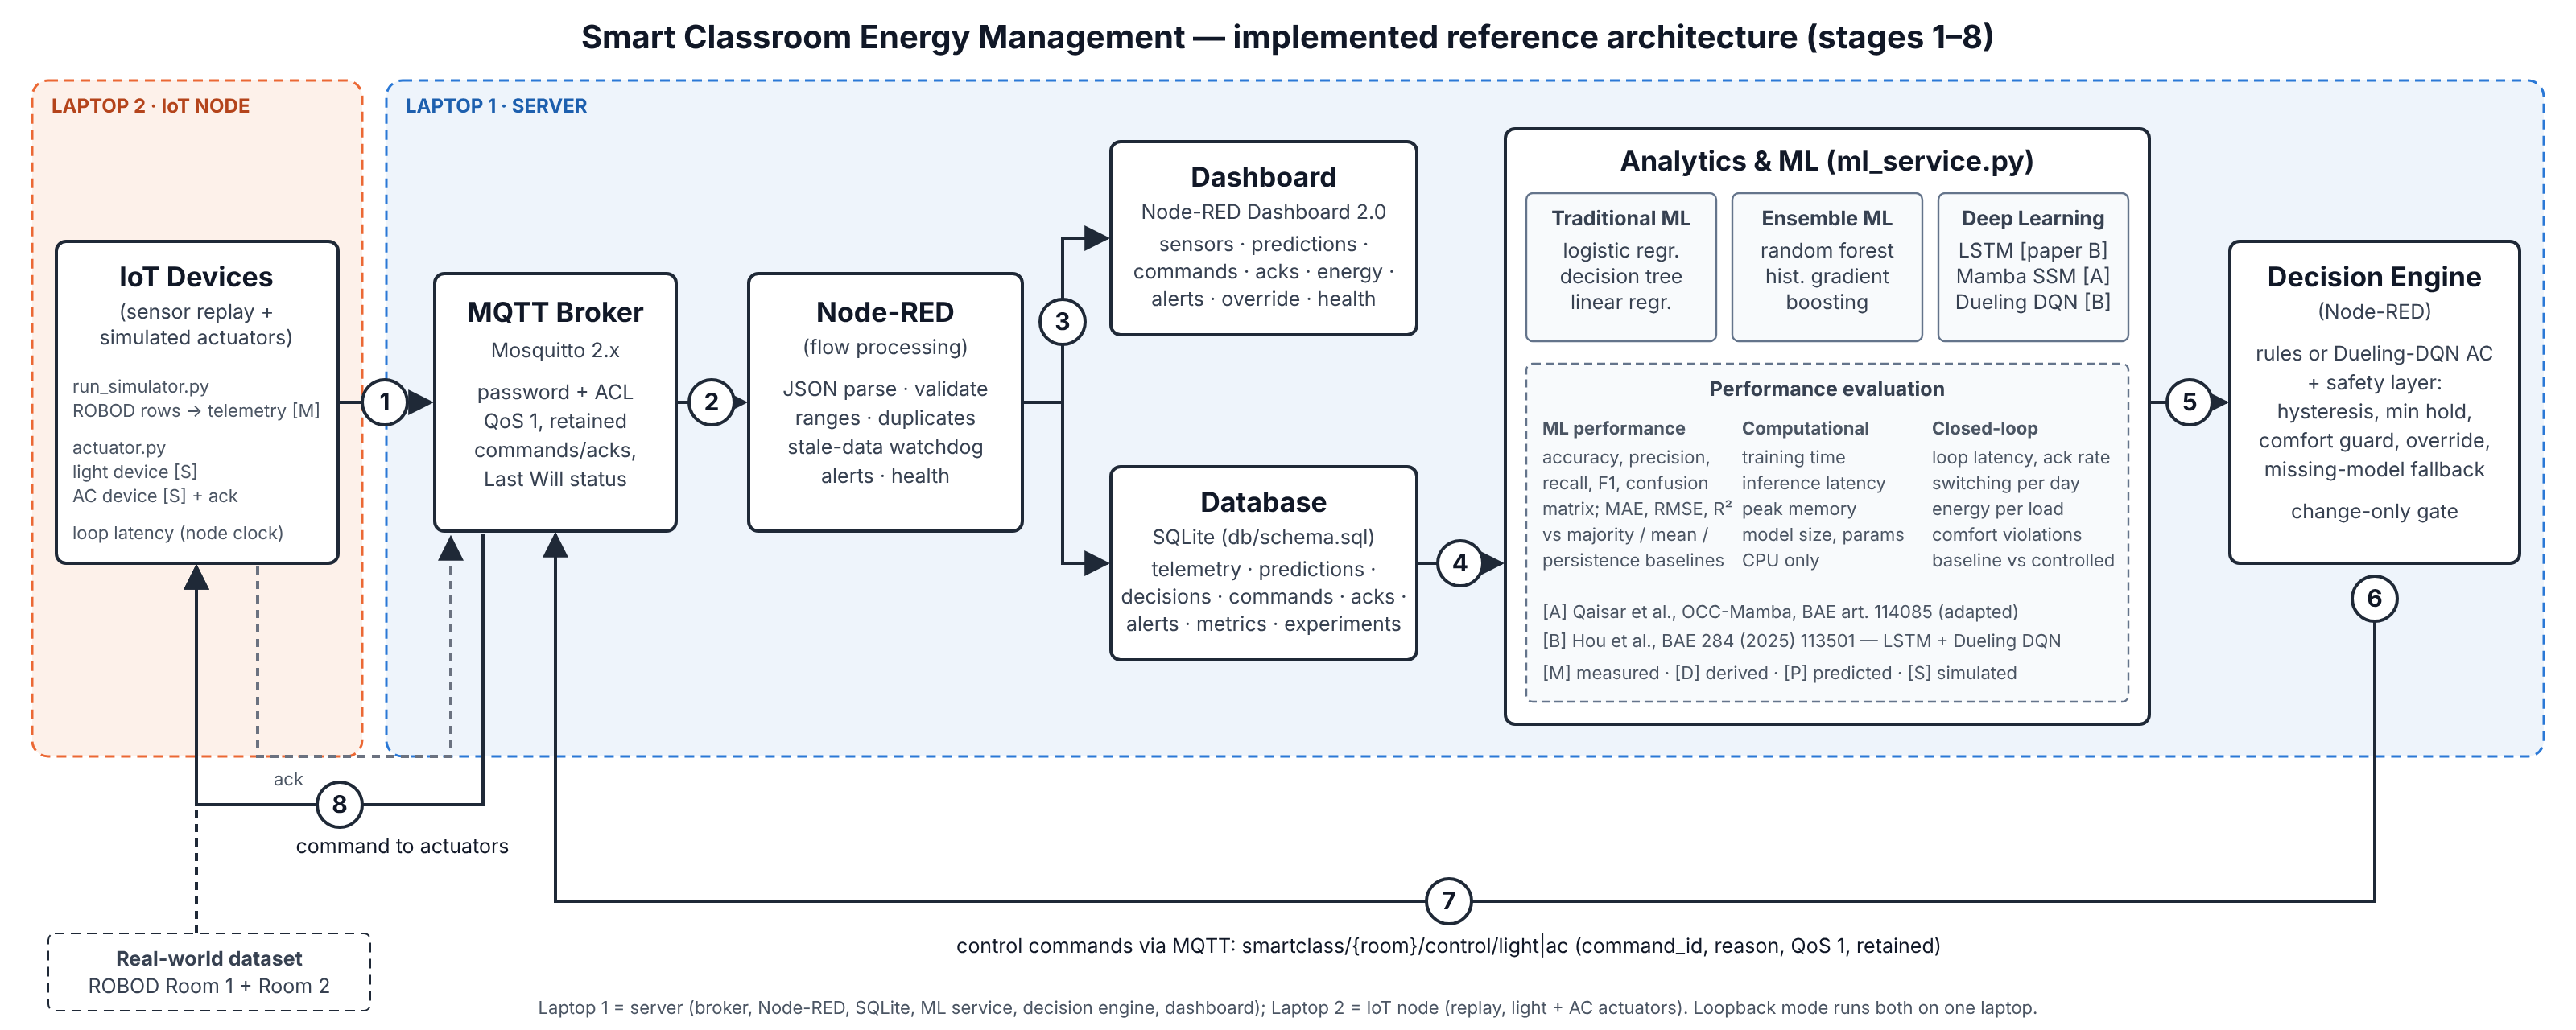
\includegraphics[width=\textwidth]{architecture.png}
\caption{Implemented architecture: eight reference stages across two laptops}
\label{fig:arch}
\end{figure}

\begin{table}[H]
\centering
\caption{Reference stages and their implementation}
\label{tab:stages}
\small
\begin{tabularx}{\textwidth}{@{}cL{3.0cm}YL{1.2cm}@{}}
\toprule
\textbf{Stage} & \textbf{Reference block} & \textbf{Implementation} & \textbf{Laptop}\\
\midrule
1 & IoT devices / dataset & \texttt{run\_simulator.py} (ROBOD rows); \texttt{actuator.py} (light + AC per room) & 2\\
2 & MQTT broker & Mosquitto: no anonymous access, password file, per-role ACL, QoS 1, retained commands/acks, Last Will & 1\\
3 & Node-RED processing & validation, duplicate drop, stale-data watchdog, alerts, device health & 1\\
4 & Database + dashboard & SQLite (8 tables); Node-RED Dashboard 2.0 & 1\\
5 & Analytics and ML & \texttt{ml\_service.py}: 6 occupancy models, arrival profile, energy forecaster, DQN recommendation & 1\\
6 & Decision engine & Node-RED ``Decision rules'': rules or Dueling DQN behind a safety layer; change-only gate & 1\\
7 & Control via MQTT & \texttt{smartclass/\{room\}/control/\{light,ac\}} with command id & 1\ra2\\
8 & Actuators + feedback & simulated state change; acknowledgement with loop latency & 2\ra1\\
\bottomrule
\end{tabularx}
\end{table}

The control logic exists once, in the Node-RED Decision rules node. The experiments and tests run that exact code.
All thresholds live in one CONFIG node, and the database schema exists once, in \texttt{db/schema.sql}.

\section{MQTT Architecture}
\begin{table}[H]
\centering
\caption{MQTT topics, direction and delivery}
\label{tab:mqtt}
\footnotesize
\begin{tabularx}{\textwidth}{@{}L{5.2cm}L{3.1cm}L{1.9cm}Y@{}}
\toprule
\textbf{Topic} & \textbf{Direction} & \textbf{QoS / retain} & \textbf{Main fields}\\
\midrule
\texttt{smartclass/\allowbreak{}\{room\}/\allowbreak{}telemetry} & node \ra{} Node-RED & 1 / no & sensors, energy [M], camera labels [M], \texttt{sent\_at\_ms}\\
\texttt{smartclass/\allowbreak{}\{room\}/\allowbreak{}validated} & Node-RED \ra{} ML & 1 / no & the validated reading\\
\texttt{smartclass/\allowbreak{}\{room\}/\allowbreak{}analytics} & ML \ra{} Node-RED & 1 / no & per-model probabilities [P], arrival, DQN action\\
\texttt{smartclass/\allowbreak{}\{room\}/\allowbreak{}control/\allowbreak{}\{light,ac\}} & Node-RED \ra{} actuator & 1 / yes & cmd, command\_id, reason\\
\texttt{smartclass/\allowbreak{}\{room\}/\allowbreak{}actuator/\allowbreak{}\{load\}} & actuator \ra{} Node-RED & 1 / yes & state, accepted, command\_id, loop latency\\
\texttt{\ldots/status} & every client & 1 / yes & online / offline (Last Will)\\
\bottomrule
\end{tabularx}
\end{table}

\textbf{Security.} Anonymous access is disabled and passwords are stored as PBKDF2-SHA512 hashes. Two roles:
\begin{itemize}
\item \texttt{sc\_server} can read and write \texttt{smartclass/\#};
\item \texttt{sc\_node} can only write telemetry, status and acknowledgements, and read control topics.
\end{itemize}
A node account therefore cannot command actuators; this is tested, and the broker logs \texttt{Denied PUBLISH}.
Clients reconnect with 1--30~s exponential back-off.

\section{Node-RED Flow}
\begin{figure}[H]
\centering
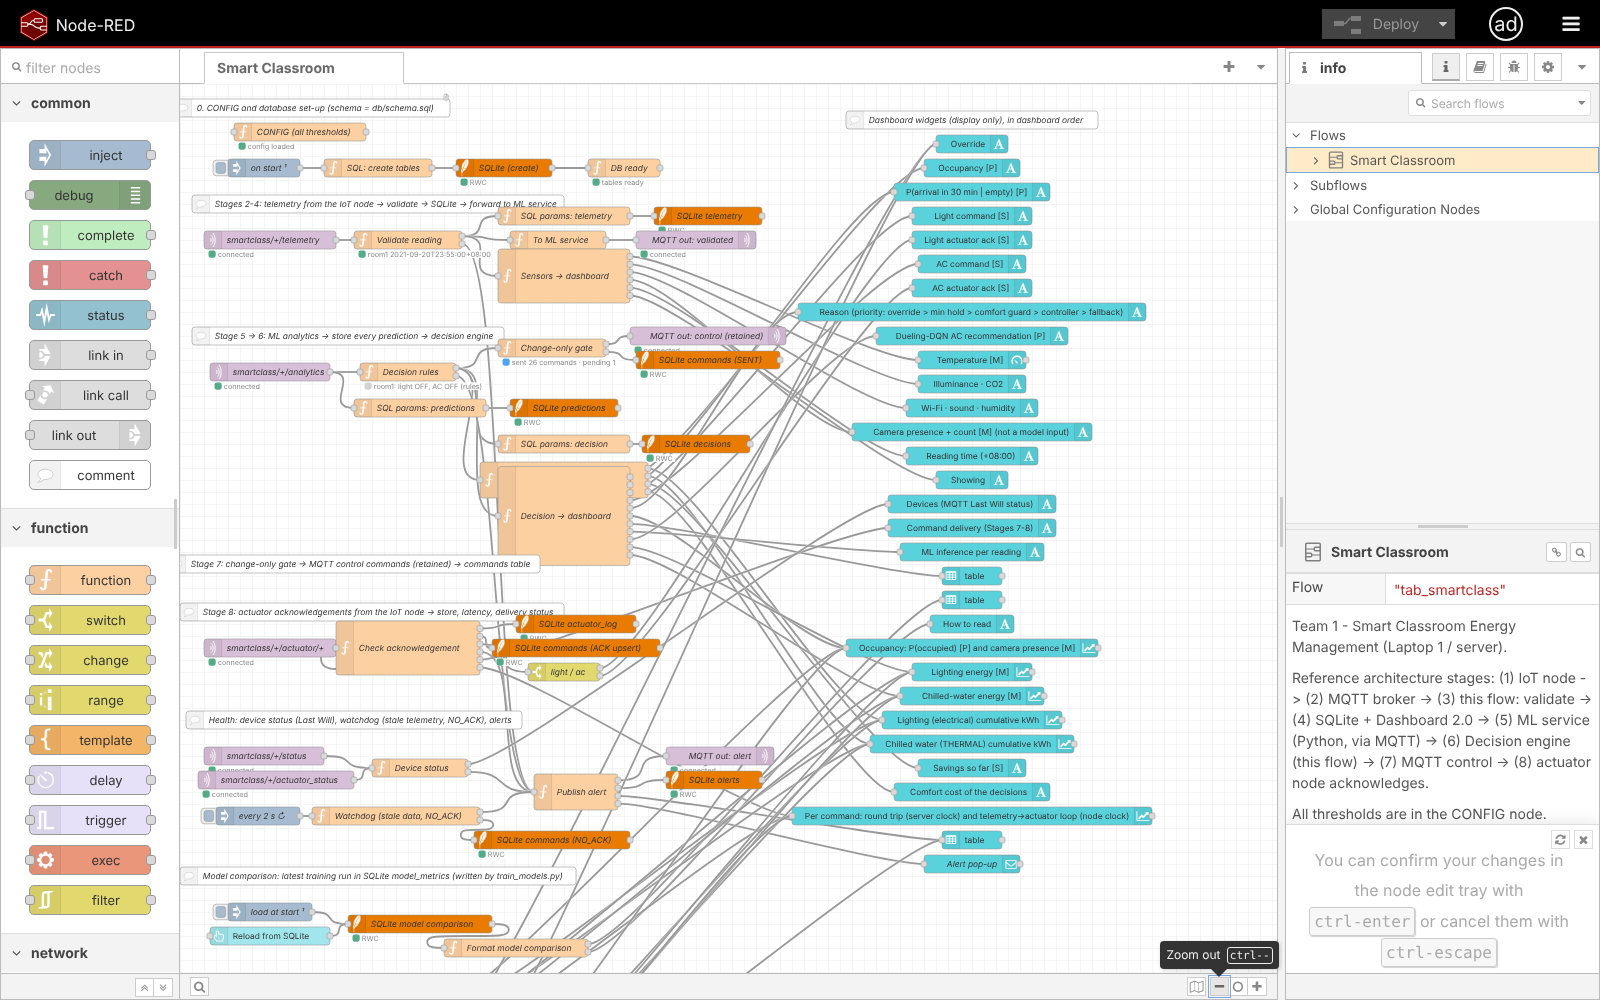
\includegraphics[width=0.92\textwidth]{nodered_flow.png}
\caption{Node-RED flow (editor, after login)}
\label{fig:nodered}
\end{figure}

The flow (118 nodes, 22 function nodes) is laid out by stage:
\begin{enumerate}
\item CONFIG (all thresholds) and table creation from the schema.
\item Telemetry \ra{} \textbf{Validate reading} (JSON, allowed room, timestamp, ranges, required fields, duplicate
  drop) \ra{} SQLite \ra{} \texttt{validated}.
\item Analytics \ra{} predictions stored \ra{} \textbf{Decision rules} \ra{} decisions stored.
\item \textbf{Change-only gate}: a command id is assigned, the command is published retained, and a SENT row is
  stored.
\item Acknowledgements \ra{} \texttt{actuator\_log} and a command upsert (ACKED, REJECTED or ACKED\_LATE), with
  round-trip and loop latency.
\item Device status (Last Will) and a watchdog every 2~s (stale telemetry after 15~s, NO\_ACK after 5~s).
\item Model-performance and offline-experiment tables loaded from SQLite.
\end{enumerate}

\textbf{Editor security.} When an editor password is set, the editor and admin API require a login; otherwise they
only answer requests from the server laptop itself.

\section{Database Design}
\begin{table}[H]
\centering
\caption{SQLite tables}
\label{tab:db}
\footnotesize
\begin{tabularx}{\textwidth}{@{}L{3.3cm}L{5.8cm}Y@{}}
\toprule
\textbf{Table} & \textbf{Key columns} & \textbf{Purpose}\\
\midrule
\texttt{telemetry} & UNIQUE(room\_id, ts) & every valid reading [M]\\
\texttt{predictions} & room, ts, model, probability, latency & every model output [P]\\
\texttt{decisions} & room, ts, light, ac, reason, controller & every decision [S]\\
\texttt{commands} & command id; status SENT, ACKED, REJECTED, NO\_ACK or ACKED\_LATE & delivery tracking\\
\texttt{actuator\_log} & room, load, state, previous, accepted & every acknowledgement\\
\texttt{alerts} & ts, room, type, message & invalid, stale, offline, no-ack, late-ack\\
\texttt{model\_metrics} & run\_id, task, model, split, metric, value & offline evaluation (imported)\\
\texttt{experiment\_results} & run\_id, experiment, scenario, metric, value, unit & registered experiments (imported)\\
\bottomrule
\end{tabularx}
\end{table}

\texttt{init\_db.py} creates the schema and imports the registered training and experiment results once per run id,
without modifying them. Python writers wait up to 15~s for a database lock and raise a visible error after that,
rather than dropping a row.

\section{Dashboard Design}
The dashboard implements all twenty required panels. Every value carries a measured [M], predicted [P] or simulated
[S] tag, every title states its unit, and live panels state their time window and data source. When data is missing,
a panel shows ``n/a'' or an instruction instead of a misleading zero. Evaluation tables are read from SQLite, not
hard-coded. The AC panel states which layer set each command, for example ``BOOST --- set by rules'' and ``DQN: OFF
--- advisory only''.

\begin{figure}[H]
\centering
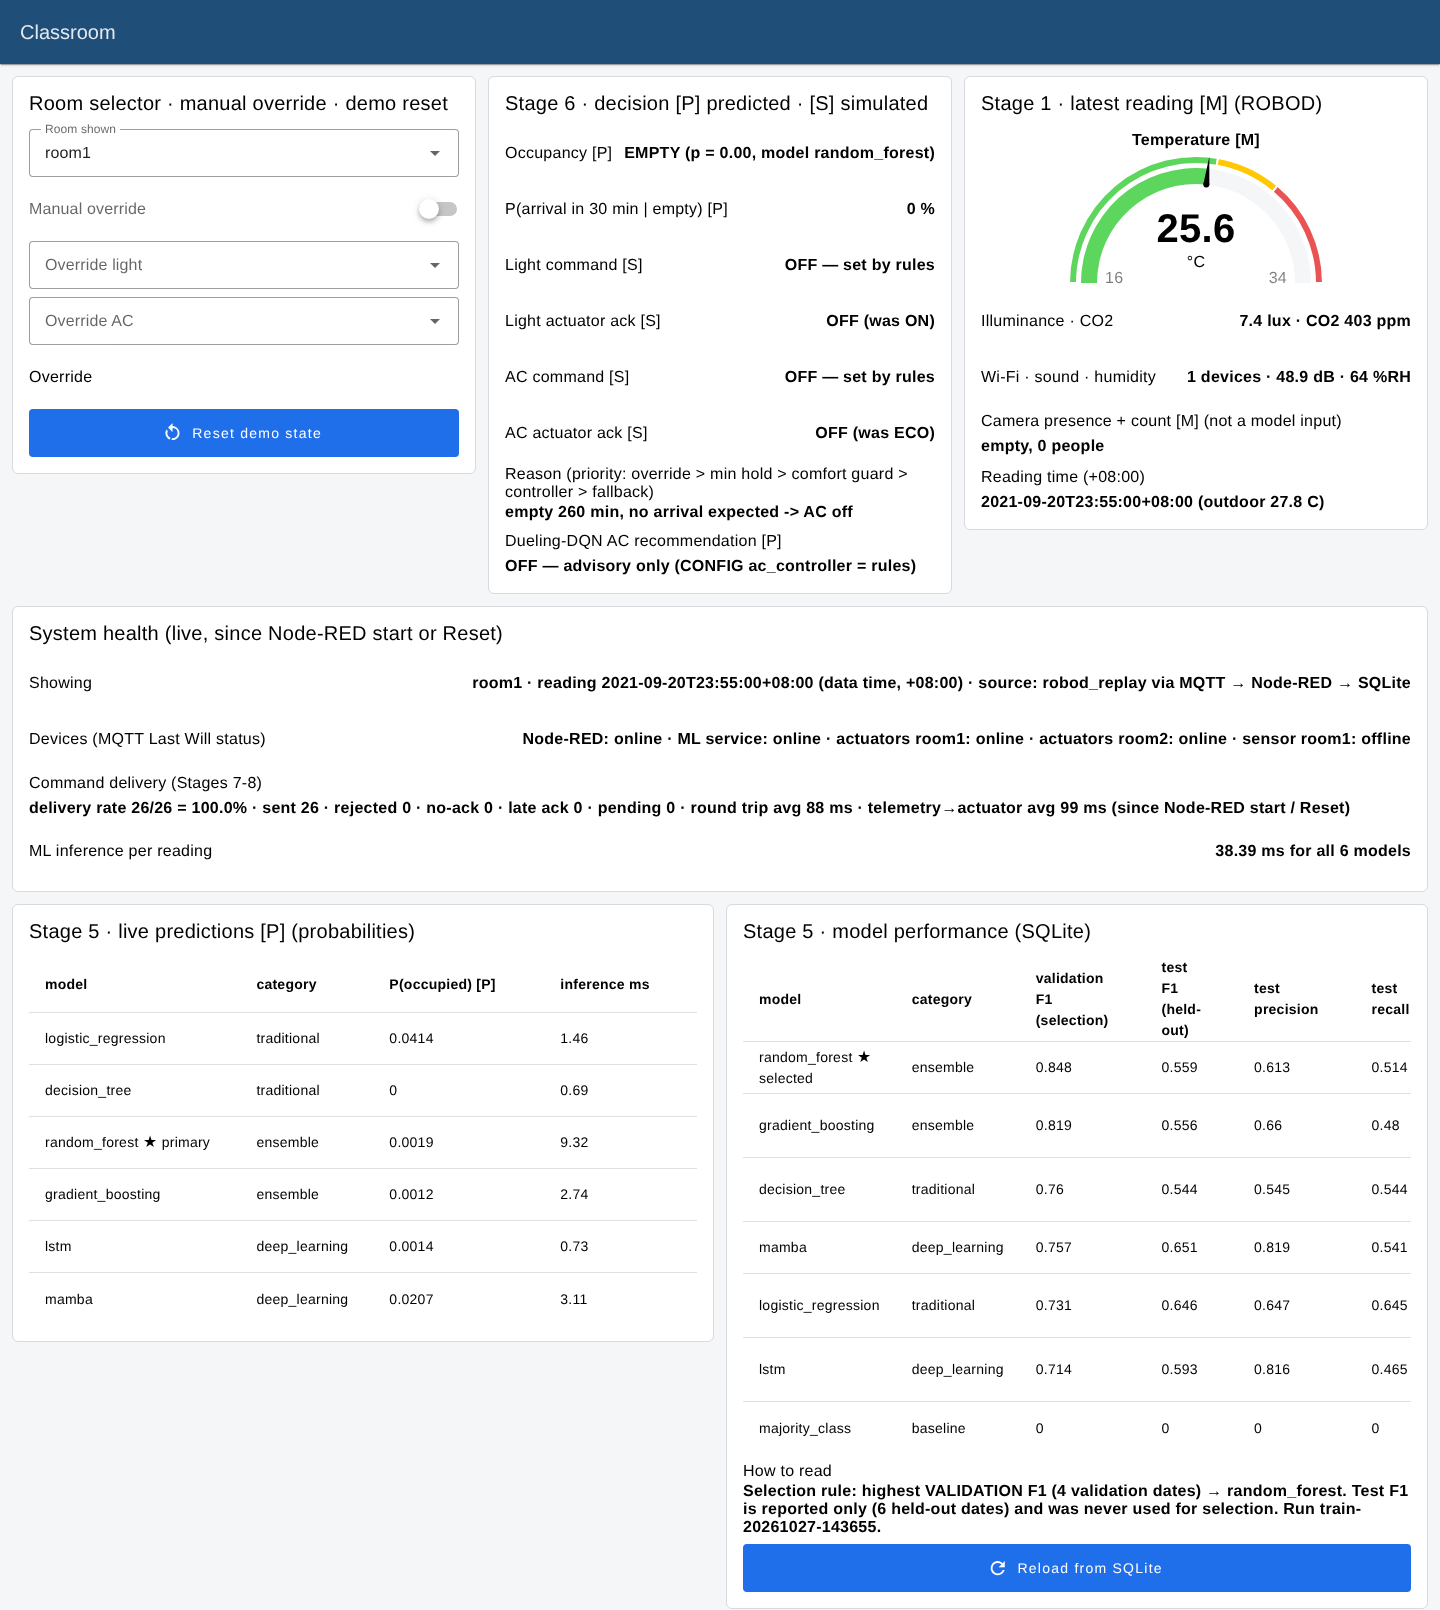
\includegraphics[width=0.85\textwidth]{dashboard_top.png}
\caption{Dashboard (1/3): control, decision with the deciding layer, sensors, health, live predictions and model performance from SQLite}
\label{fig:dash1}
\end{figure}

\begin{figure}[H]
\centering
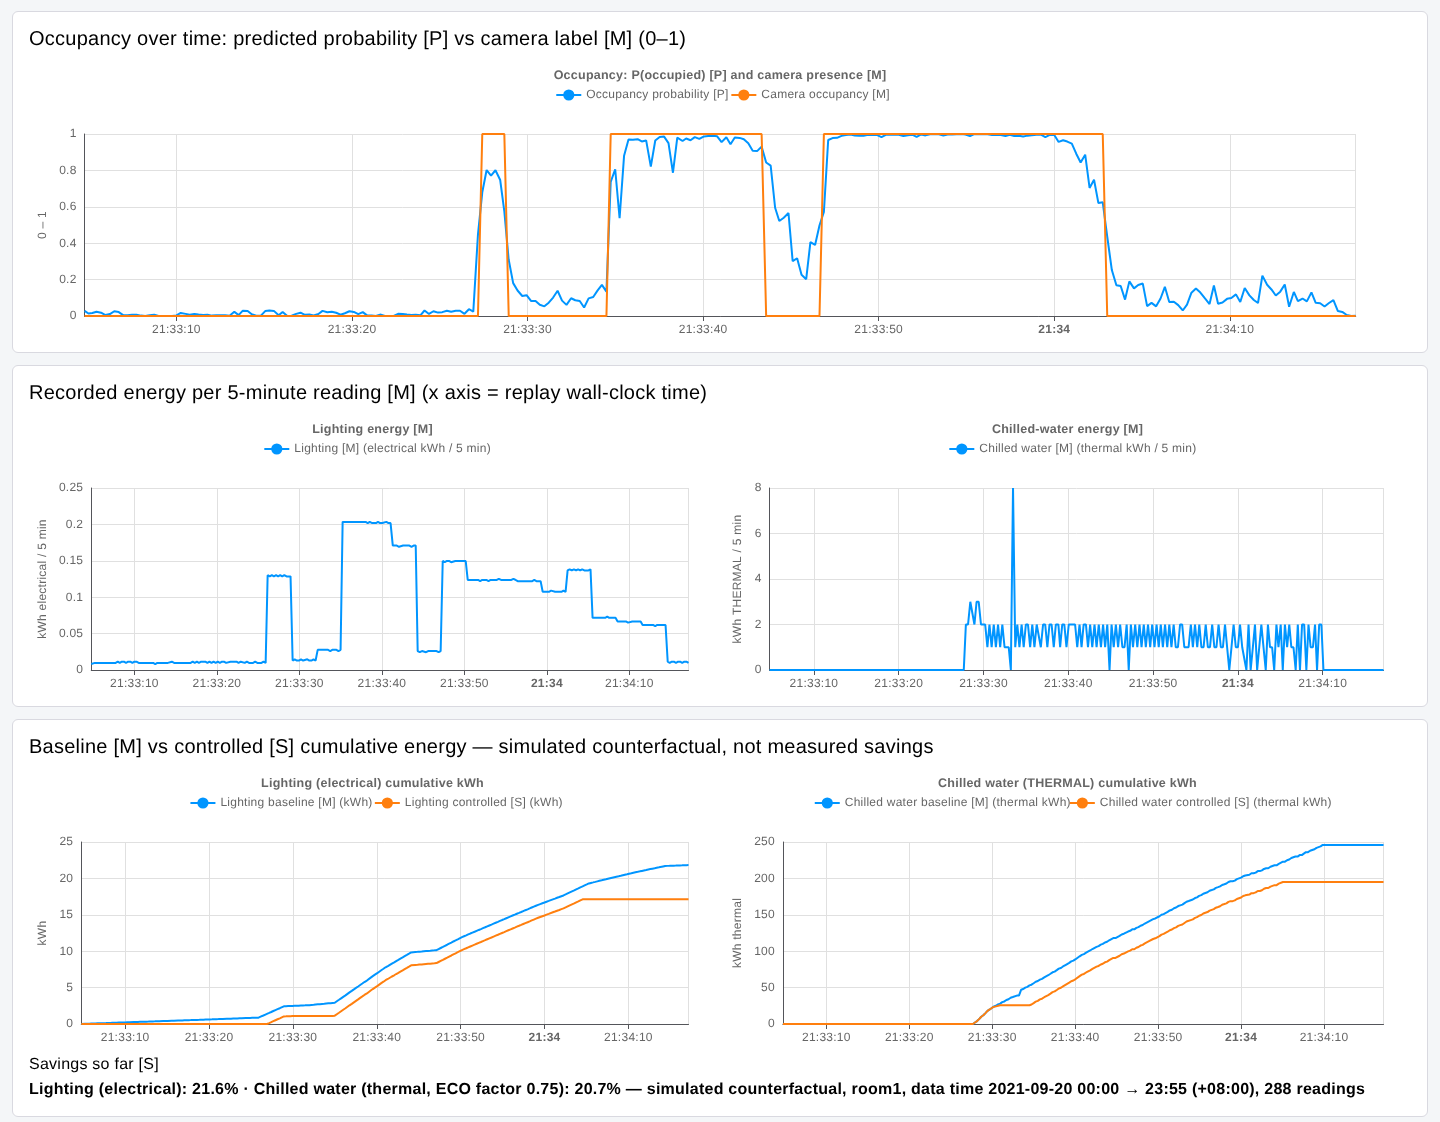
\includegraphics[width=0.85\textwidth]{dashboard_charts.png}
\caption{Dashboard (2/3): occupancy [P] vs camera [M], recorded energy [M], baseline [M] vs controlled [S] cumulative energy}
\label{fig:dash2}
\end{figure}

\begin{figure}[H]
\centering
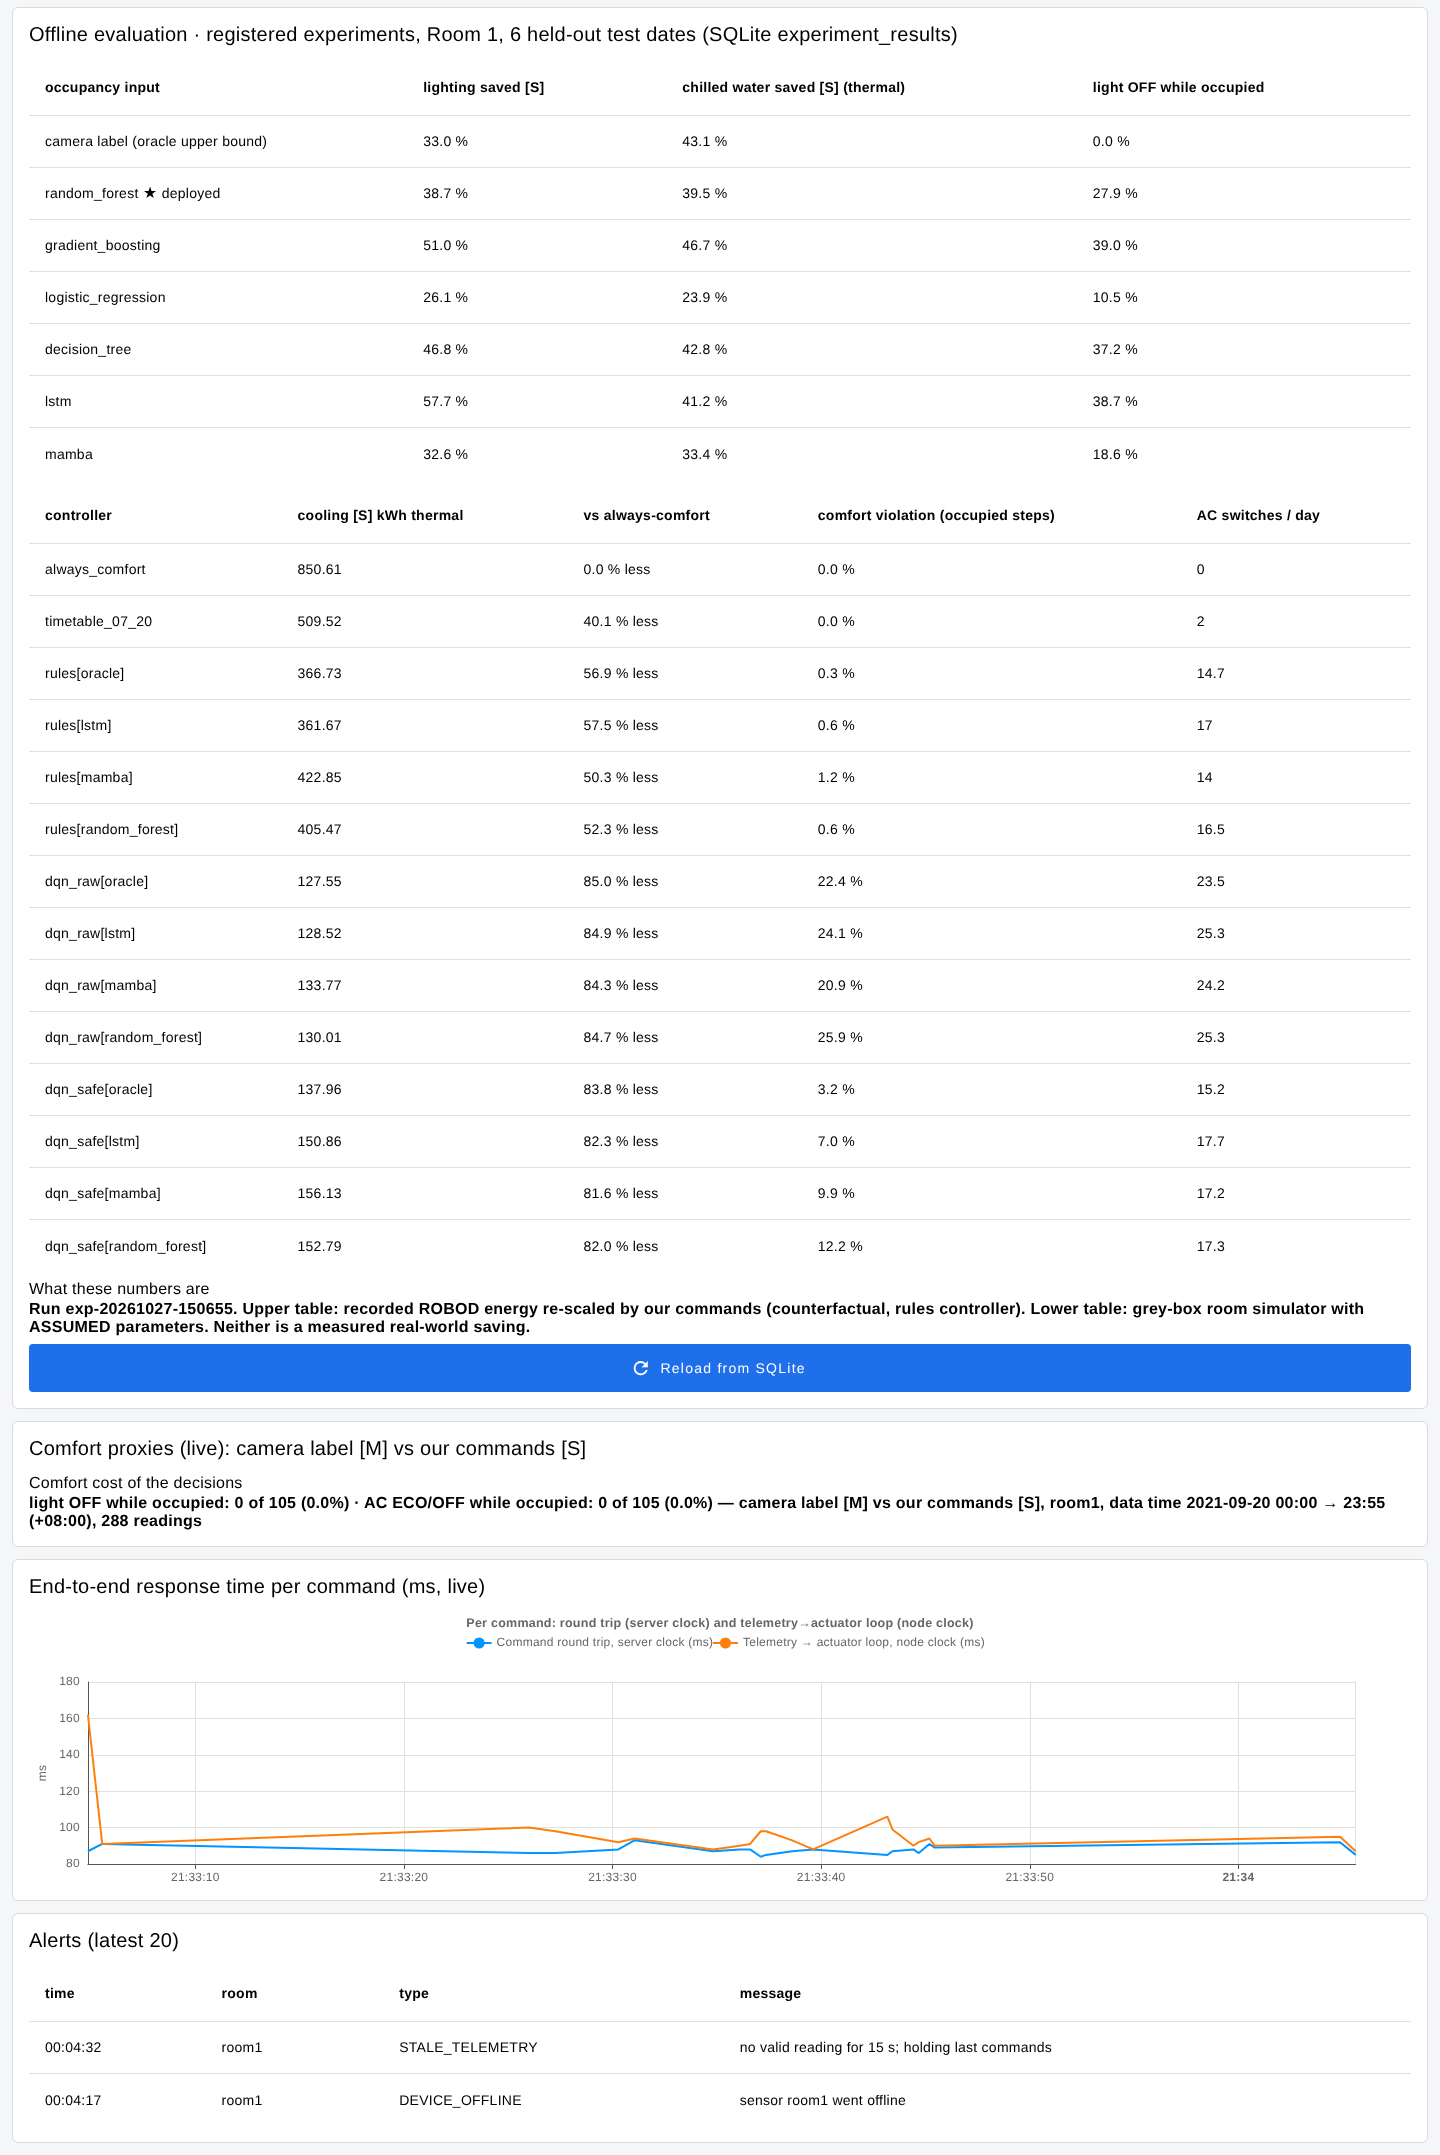
\includegraphics[width=0.85\textwidth,height=0.55\textheight,keepaspectratio]{dashboard_offline.png}
\caption{Dashboard (3/3): registered offline experiments from SQLite, live comfort proxies, response time and alerts}
\label{fig:dash3}
\end{figure}

\section{Feature Engineering}
\begin{itemize}
\item \textbf{Sensors} (time $t$): Wi-Fi devices, \COtwo{}, sound, humidity, temperature, illuminance.
\item \textbf{Time:} sine and cosine of the time of day, and weekday.
\item \textbf{Tabular extras:} Wi-Fi 30-minute mean, \COtwo{} change over 15 and 55 minutes, 30-minute maximum
  sound, 15-minute temperature change.
\item \textbf{Sequences:} the last 12 readings (1~hour) of the 9 sensor and time features.
\end{itemize}

\textbf{Leakage controls} (all tested): features use only time $\leq t$; splits are by whole date; scalers are fitted
on training dates only; camera labels are never inputs; live features equal offline features.

\section{Machine-Learning Models}
\begin{table}[H]
\centering
\caption{Occupancy and energy models}
\label{tab:models}
\small
\begin{tabularx}{\textwidth}{@{}L{3.2cm}L{2.4cm}Y@{}}
\toprule
\textbf{Model} & \textbf{Category} & \textbf{Settings}\\
\midrule
Majority class & baseline & always predicts ``empty''\\
Logistic regression & traditional & standardised, class-balanced\\
Decision tree & traditional & depth 5, class-balanced\\
Random forest & ensemble & 200 trees, minimum leaf 5, class-balanced, seed 42\\
Gradient boosting & ensemble & histogram gradient boosting, 200 iterations, learning rate 0.05\\
LSTM (paper B) & deep learning & 1 layer, 32 units, last hidden state \ra{} logit; 5,537 parameters\\
Mamba (paper A family) & deep learning & embedding 32, two pre-norm residual Mamba blocks; 17,217 parameters\\
Energy forecasters & regression & linear regression, random forest, gradient boosting vs mean and persistence baselines\\
\bottomrule
\end{tabularx}
\end{table}

\textbf{Deep-learning training.} Adam (learning rate $10^{-3}$), class-weighted binary cross-entropy and early
stopping on validation F1. Each Mamba block has: expand 2, a causal depth-wise convolution (kernel 4), SiLU,
input-dependent $\Delta$/$B$/$C$ (state size 8), zero-order-hold discretisation, a selective scan, a $D$ skip
connection and SiLU gating. It is written in plain PyTorch, with no CUDA kernel.

\section{Research-Paper Adaptations}
\begin{table}[H]
\centering
\caption{What was taken from each paper and what was adapted}
\label{tab:adapt}
\small
\begin{tabularx}{\textwidth}{@{}L{3.0cm}L{3.4cm}L{3.6cm}Y@{}}
\toprule
\textbf{Aspect} & \textbf{Paper} & \textbf{Ours} & \textbf{Why}\\
\midrule
A: architecture & OCC-Mamba (configuration not accessible) & generic Mamba blocks & full text unavailable\\
B: occupancy labels & \COtwo{} change-point labels & ROBOD camera labels & ground truth exists\\
B: LSTM inputs & \COtwo{} & 6 sensors + time & richer signals available\\
B: DRL state/action/reward & not accessible & our own design & declared openly\\
B: plant & their simulation platform & grey-box RC thermal + \COtwo{} model & ROBOD cannot identify the plant\\
B: deployment & -- & DQN behind a safety layer; rules default & comfort results\\
\bottomrule
\end{tabularx}
\end{table}

Neither paper is reproduced exactly; both are research-inspired adaptations.

\section{Decision Engine}
\textbf{Priority order} (highest first), recorded for every decision:
\begin{enumerate}
\item manual override;
\item minimum-hold time;
\item comfort safety guard;
\item selected AC controller (rules by default, or the DQN);
\item missing-model fallback.
\end{enumerate}

\textbf{Rules:}
\begin{itemize}
\item \textbf{Hysteresis:} a room becomes occupied at $p \geq 0.25$ and empty only at $p < 0.15$. These values were
  tuned on the validation dates; the earlier 0.6/0.4 switched lights off in 22.5\% of occupied validation intervals,
  while 0.25/0.15 does so in 13.7\%.
\item \textbf{Occupied:} light ON (DIM above 300~lux in Room~2 only), AC COMFORT, or BOOST above 25.5~°C.
\item \textbf{Empty:} a 15-minute grace period, then light OFF and AC ECO; AC OFF after 30 minutes if no arrival is
  expected.
\item \textbf{PRECOOL:} when the arrival probability within 30 minutes is at least 0.2 and the room is more than
  0.5~°C above comfort.
\item \textbf{Minimum hold:} 10 minutes for downward switches; switching up for an occupied room is immediate.
\item \textbf{Start-up:} an empty room is never switched ON.
\item \textbf{No model output:} hold the last commands, else use the 08:00--20:00 timetable.
\end{itemize}

\textbf{The ``AC BOOST while the DQN says OFF'' case.} In the default rules mode the DQN is advisory only. The rules
chose BOOST because the room was occupied above 25.5~°C, and the dashboard now says so. The safety layer is never
bypassed in favour of the DQN.

\section{Dueling DQN}
\begin{itemize}
\item \textbf{Network:} $Q(s,a) = V(s) + A(s,a) - \overline{A}(s)$, with two hidden layers of 64 ReLU units; 24~kB on
  disk; 0.12~ms per decision.
\item \textbf{State:} LSTM occupancy probability, arrival probability, temperature, \COtwo{}, outdoor temperature,
  time of day.
\item \textbf{Actions:} OFF, ECO, COMFORT, BOOST.
\item \textbf{Reward per 5 minutes:} $-(\text{cooling kWh}/3.5 + \text{fan kWh}) - 0.5\times$K outside 23--26~°C
  $- 0.3\times(\text{\COtwo{}} - 1000)/100$. The comfort and \COtwo{} terms apply only while the room is occupied.
\item \textbf{Training:} replay buffer 50k, target network synchronised every 1,000 steps, $\varepsilon$ from 1 to
  0.05, $\gamma = 0.97$, Huber loss, 400 one-day episodes on training and validation dates (219~s on CPU). The
  occupancy input is out-of-fold LSTM output, to avoid in-sample optimism.
\end{itemize}

\textbf{Simulator.} A first-order RC model with an ideal thermostat per mode (ECO 26, COMFORT 24, BOOST 23~°C) and a
\COtwo{} mass balance, driven by ROBOD's outdoor temperature, solar radiation, outdoor \COtwo{} and occupant counts.
The parameters are assumed and declared, and were calibrated so that the free-running room peaks around 30~°C and
24/7 COMFORT uses about 140~kWh thermal per day (ROBOD median 132).

\begin{figure}[H]
\centering
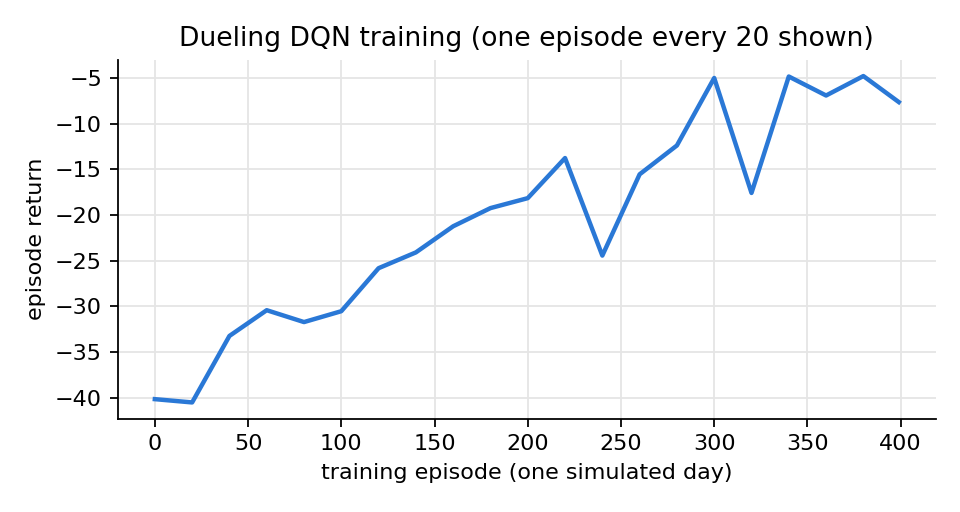
\includegraphics[width=0.62\textwidth]{dqn_training.png}
\caption{Dueling DQN training return over 400 episodes}
\label{fig:dqn}
\end{figure}

\section{Actuator Simulation}
\texttt{actuator.py} runs on Laptop~2, one process per room, controlling two loads: light (ON/DIM/OFF) and AC
(OFF/ECO/COMFORT/BOOST/PRECOOL). For each command it validates the value, applies it to the simulated state, and
publishes a retained acknowledgement with the state, previous state, acceptance, command id and loop latency
(measured on the node's own clock). An unknown command is rejected and raises an alert. No physical actuator was
tested.

\section{Experimental Methodology}
\begin{table}[H]
\centering
\caption{Experiments and their protocols}
\label{tab:exp}
\small
\begin{tabularx}{\textwidth}{@{}L{3.3cm}Y@{}}
\toprule
\textbf{Experiment} & \textbf{Protocol}\\
\midrule
Occupancy models & train on 19 dates; select and tune on 4 validation dates; report on 6 test dates; 5-fold GroupKFold by date; Room~2 cross-room\\
Test-set uncertainty & saved models re-predict the test dates (F1 reproduced exactly); 2,000$\times$ date-cluster bootstrap (seed 42), paired difference vs the primary model\\
Energy forecasting & next 5 minutes, test dates, vs mean and persistence baselines\\
Recorded counterfactual & recorded energy $\times$ our command (light OFF 0, DIM 0.5; AC OFF 0, ECO 0.75), per occupancy source; sensitivity ECO 0.5--0.9\\
Closed-loop simulation & 6 test days in the grey-box room; always-on, timetable, rules, raw DQN, DQN + safety; occupancy from camera, LSTM, Mamba or RF\\
DQN reward weight & 150 episodes, camera occupancy, raw policy, 6 test dates (shortened protocol)\\
Live closed loop & full-day replay through MQTT, Node-RED, ML and actuators; metrics from SQLite\\
\bottomrule
\end{tabularx}
\end{table}

Test dates were never used for training, selection or tuning, and all seeds are 42.

% ---------------------------------------------------------------- Chapter 5
\chapter{Results and Discussion}\label{ch:results}

\section{Model Evaluation}
\begin{figure}[H]
\centering
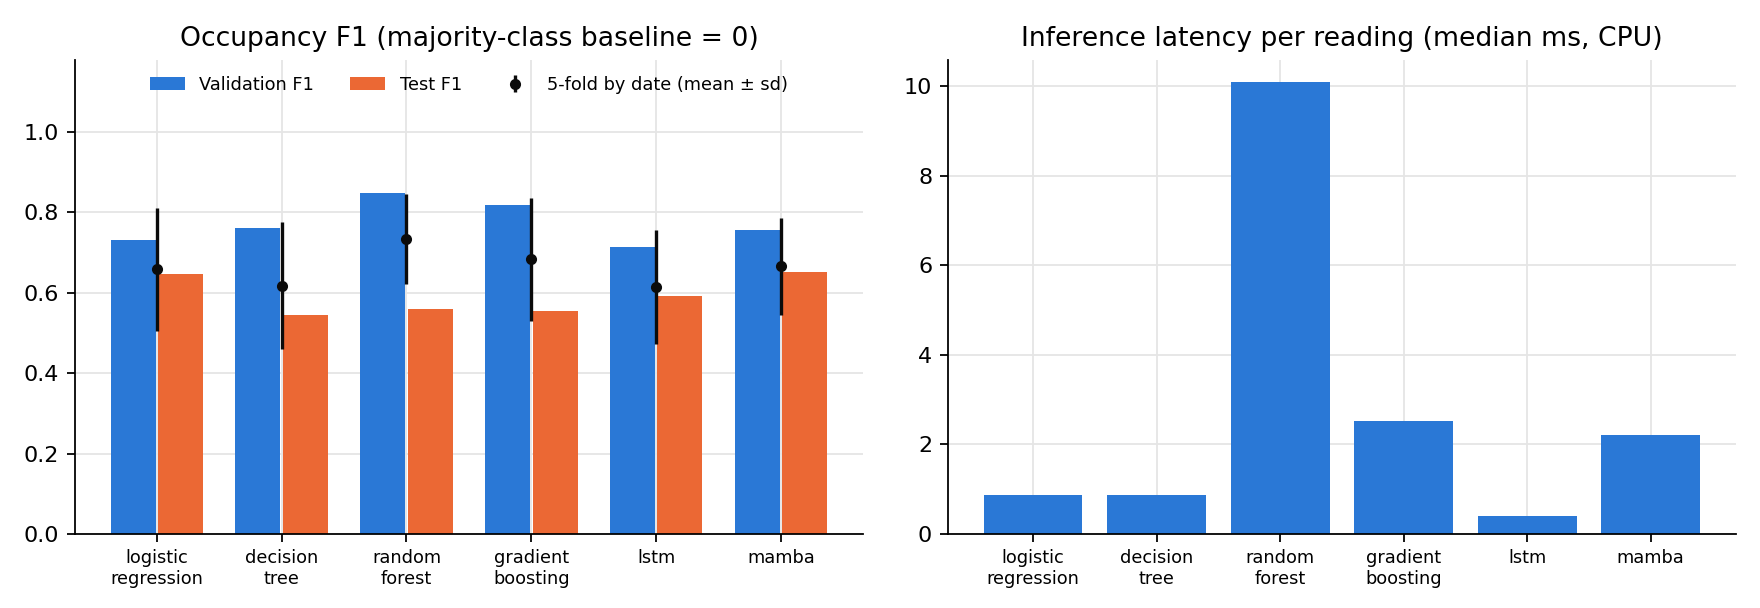
\includegraphics[width=\textwidth]{model_comparison.png}
\caption{Occupancy model comparison: F1 by split and inference latency}
\label{fig:models}
\end{figure}

\begin{table}[H]
\centering
\caption{Occupancy results, Room 1 (test F1 with 95\% date-cluster bootstrap interval)}
\label{tab:occ}
\footnotesize
\setlength{\tabcolsep}{4pt}
\begin{tabularx}{\textwidth}{@{}L{2.4cm}cccL{3.0cm}ccc@{}}
\toprule
\textbf{Model} & \textbf{Val F1} & \textbf{Test acc.} & \textbf{Test P / R} & \textbf{Test F1 [95\% CI]} & \textbf{CV F1} & \textbf{Room 2 F1} & \textbf{Latency (ms)}\\
\midrule
Majority class & 0.000 & 0.800 & 0 / 0 & 0.000 & 0.00 & 0.000 & 0.02\\
Logistic regression & 0.731 & 0.859 & 0.65 / 0.65 & 0.646 [0.34, 0.77] & 0.66 $\pm$ 0.15 & 0.679 & 0.88\\
Decision tree & 0.760 & 0.818 & 0.55 / 0.54 & 0.544 [0.20, 0.77] & 0.62 $\pm$ 0.16 & 0.657 & 0.86\\
\textbf{Random forest} & \textbf{0.848} & 0.838 & 0.61 / 0.51 & 0.559 [0.19, 0.78] & \textbf{0.73 $\pm$ 0.11} & 0.667 & 10.1\\
Gradient boosting & 0.819 & 0.846 & 0.66 / 0.48 & 0.556 [0.14, 0.77] & 0.68 $\pm$ 0.15 & 0.635 & 2.5\\
LSTM (B) & 0.714 & 0.872 & 0.82 / 0.47 & 0.593 [0.06, 0.81] & 0.61 $\pm$ 0.14 & 0.637 & 0.40\\
Mamba (A) & 0.757 & \textbf{0.884} & 0.82 / 0.54 & \textbf{0.651} [0.30, 0.78] & 0.67 $\pm$ 0.12 & 0.570 & 2.2\\
\bottomrule
\end{tabularx}
\end{table}

\begin{figure}[H]
\centering
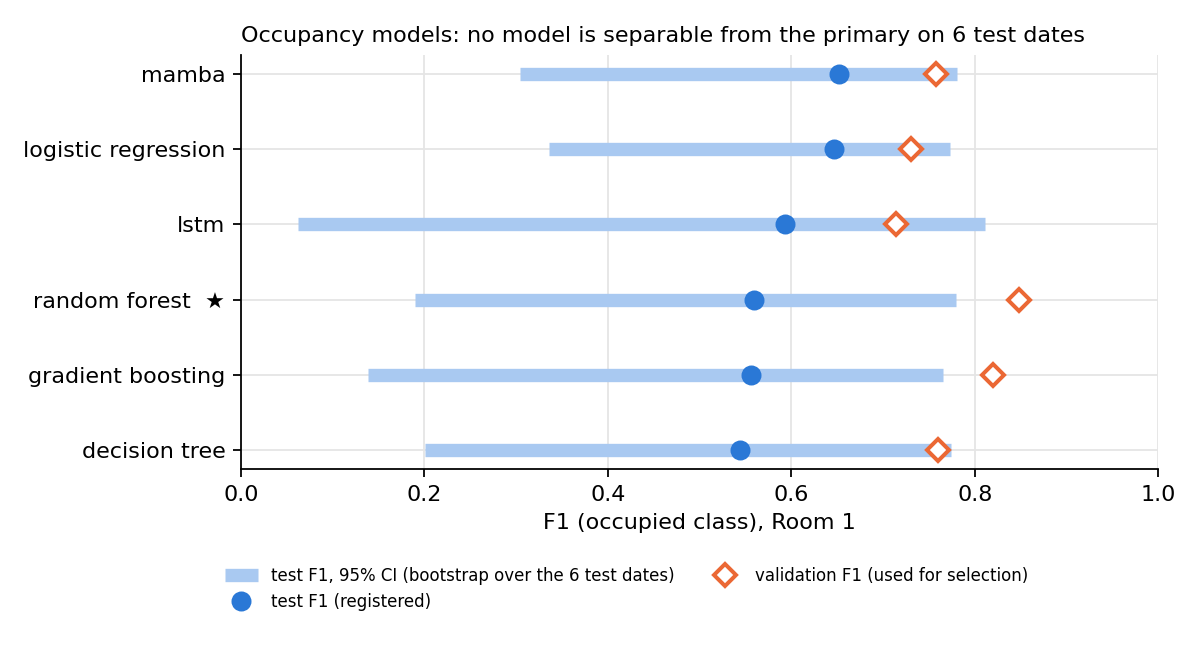
\includegraphics[width=0.8\textwidth]{bootstrap_ci_test_f1.png}
\caption{Test F1 with 95\% date-cluster bootstrap intervals and the validation F1 used for selection}
\label{fig:ci}
\end{figure}

\textbf{Why the random forest is the primary model.}
\begin{itemize}
\item It was chosen by the rule fixed in advance: the highest validation F1 (0.848). It also had the best 5-fold CV
  F1 (0.73 $\pm$ 0.11).
\item Mamba scores higher on test, but re-selecting by test F1 would be test-set selection, which would make the test
  score optimistic.
\item The paired bootstrap shows the gap is not significant: Mamba $-$ RF $= +0.093$ F1, 95\% CI $[-0.18, +0.38]$.
  Every model's interval against the random forest includes zero.
\item Two test days have 0 and 1 occupied intervals, which widens the intervals.
\end{itemize}

All models are far above the majority baseline. The deep models are the most precise (0.82) but miss about half of
the occupied intervals. Every model runs in at most 15~ms per reading (p95) on one CPU thread.

\begin{table}[H]
\centering
\caption{Energy forecasting, next 5 minutes, test dates}
\label{tab:energy}
\footnotesize
\begin{tabular}{@{}lcccc@{}}
\toprule
\textbf{Model} & \textbf{Lighting MAE (kWh)} & \textbf{Lighting $R^2$} & \textbf{Chilled-water MAE (kWh th)} & \textbf{Chilled-water $R^2$}\\
\midrule
Mean baseline & 0.0539 & $-0.00$ & 0.669 & $-0.02$\\
Persistence & \textbf{0.0022} & 0.965 & 0.450 & $-0.09$\\
Linear regression & 0.0028 & \textbf{0.966} & 0.466 & 0.32\\
Random forest & 0.0144 & 0.836 & 0.244 & 0.66\\
Gradient boosting & 0.0040 & \textbf{0.966} & \textbf{0.243} & \textbf{0.70}\\
\bottomrule
\end{tabular}
\end{table}

For lighting, nothing beats persistence: the lights rarely change between 5-minute steps. For chilled water, the
ensembles halve the error of both baselines. The pre-cooling arrival profile caught 7 of 47 arrivals with 158 false
alarms (F1 0.066): it works as designed, but it is weak.

\section{Energy Evaluation}
All numbers in this section are \textbf{simulated}; none is a measured saving in a real building.

\begin{figure}[H]
\centering
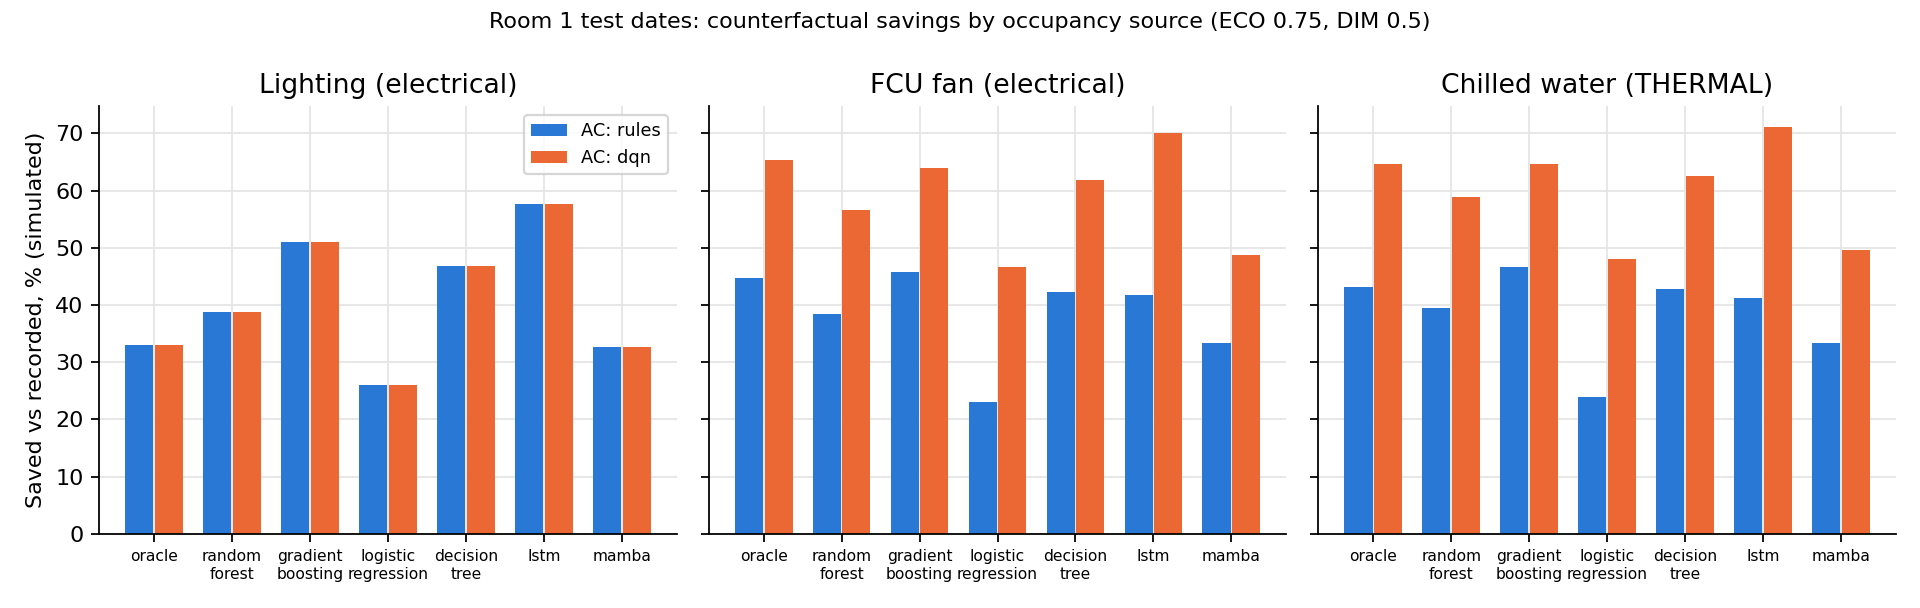
\includegraphics[width=\textwidth]{savings_by_source.png}
\caption{Recorded-energy counterfactual savings by occupancy source (Room 1 test dates)}
\label{fig:savings}
\end{figure}

\begin{table}[H]
\centering
\caption{Recorded-energy counterfactual, Room 1, 6 test dates, rules (ECO 0.75, DIM 0.5)}
\label{tab:cf}
\footnotesize
\setlength{\tabcolsep}{4pt}
\begin{tabular}{@{}lcccc@{}}
\toprule
\textbf{Occupancy input} & \textbf{Lighting} & \textbf{Chilled water (th)} & \textbf{FCU fan} & \textbf{Lights OFF while occupied}\\
\midrule
Camera label (upper bound) & 33.0\% & 43.1\% & 44.7\% & 0 / 344\\
\textbf{Random forest (deployed)} & 38.7\% & 39.5\% & 38.4\% & 96 / 344 (27.9\%)\\
Logistic regression & 26.1\% & 23.9\% & 23.0\% & 36 / 344 (10.5\%)\\
Mamba & 32.6\% & 33.4\% & 33.3\% & 64 / 344 (18.6\%)\\
LSTM & 57.7\% & 41.2\% & 41.8\% & 133 / 344 (38.7\%)\\
\bottomrule
\end{tabular}
\end{table}

Savings above the camera bound come from switching off occupied rooms; they are a comfort cost, not a real saving.
Chilled-water savings change by less than 1.5 points across ECO factors 0.5--0.9, because most of the saving comes
from switching the AC off.

\begin{table}[H]
\centering
\caption{Closed-loop simulation, 6 test days (AC only)}
\label{tab:cl}
\footnotesize
\setlength{\tabcolsep}{3pt}
\resizebox{\textwidth}{!}{%
\begin{tabular}{@{}lcccccc@{}}
\toprule
\textbf{Controller} & \textbf{Cooling kWh\textsubscript{th}} & \textbf{vs always-on} & \textbf{Fan kWh\textsubscript{e}} & \textbf{Outside 23--26 °C} & \textbf{K$\cdot$h} & \textbf{Switches/day}\\
\midrule
Always COMFORT & 850.6 & -- & 37.5 & 0.0\% & 0.00 & 0.0\\
Timetable 07--20 & 509.5 & $-40.1$\% & 20.3 & 0.0\% & 0.00 & 2.0\\
Rules + camera (bound) & 366.7 & $-56.9$\% & 12.3 & 0.3\% & 0.01 & 14.7\\
Rules + LSTM & 361.7 & $-57.5$\% & 12.3 & 0.6\% & 0.07 & 17.0\\
Rules + Mamba & 422.9 & $-50.3$\% & 15.1 & 1.2\% & 0.08 & 14.0\\
\textbf{Rules + RF (default)} & \textbf{405.5} & $\mathbf{-52.3}$\textbf{\%} & 14.2 & \textbf{0.6\%} & 0.07 & 16.5\\
DQN raw + LSTM & 128.5 & $-84.9$\% & 2.3 & 24.1\% & 3.13 & 25.3\\
DQN + safety + LSTM & 150.9 & $-82.3$\% & 2.8 & 7.0\% & 0.59 & 17.7\\
DQN + safety + RF & 152.8 & $-82.0$\% & 2.7 & 12.2\% & 1.20 & 17.3\\
\bottomrule
\end{tabular}}
\end{table}

\begin{figure}[H]
\centering
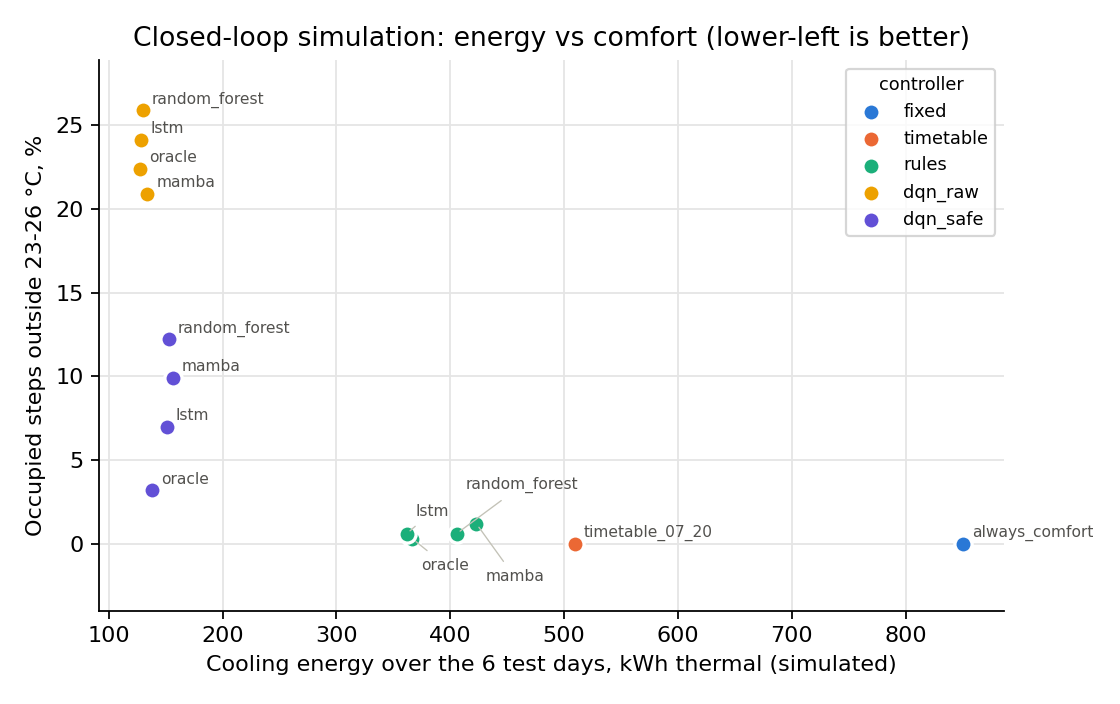
\includegraphics[width=0.72\textwidth]{closed_loop_tradeoff.png}
\caption{Energy vs comfort trade-off in the closed-loop simulation}
\label{fig:tradeoff}
\end{figure}

\section{Comfort Analysis}
\begin{itemize}
\item \textbf{Rules:} 0.6\% of occupied intervals fall outside 23--26~°C with the deployed model, close to the 0.3\%
  camera bound. \COtwo{} never exceeded 1,000~ppm in any scenario, so the air-quality term was never binding.
\item \textbf{Lighting} is the real comfort weakness of predicted occupancy: lights were wrongly OFF in 27.9\% of
  occupied intervals on the test dates with the deployed model (13.7\% on validation, 8.1\% on Room~2). A deployment
  would need a motion sensor or a minimum-lighting fallback.
\item \textbf{DQN:} the raw policy leaves occupied rooms warm (24.1\% violations); the safety layer cuts this to
  7.0\%. Raising the comfort weight from 0.5 to 2.0 (shortened protocol) cut violations from 26.5\% to 1.7\% for 5\%
  more cooling (115.7 \ra{} 121.6~kWh thermal). The problem is the reward weighting.
\item \textbf{Live:} during the 2021-09-20 replay, 0 of 105 occupied readings had the lights OFF or the AC in ECO/OFF.
\end{itemize}

\begin{figure}[H]
\centering
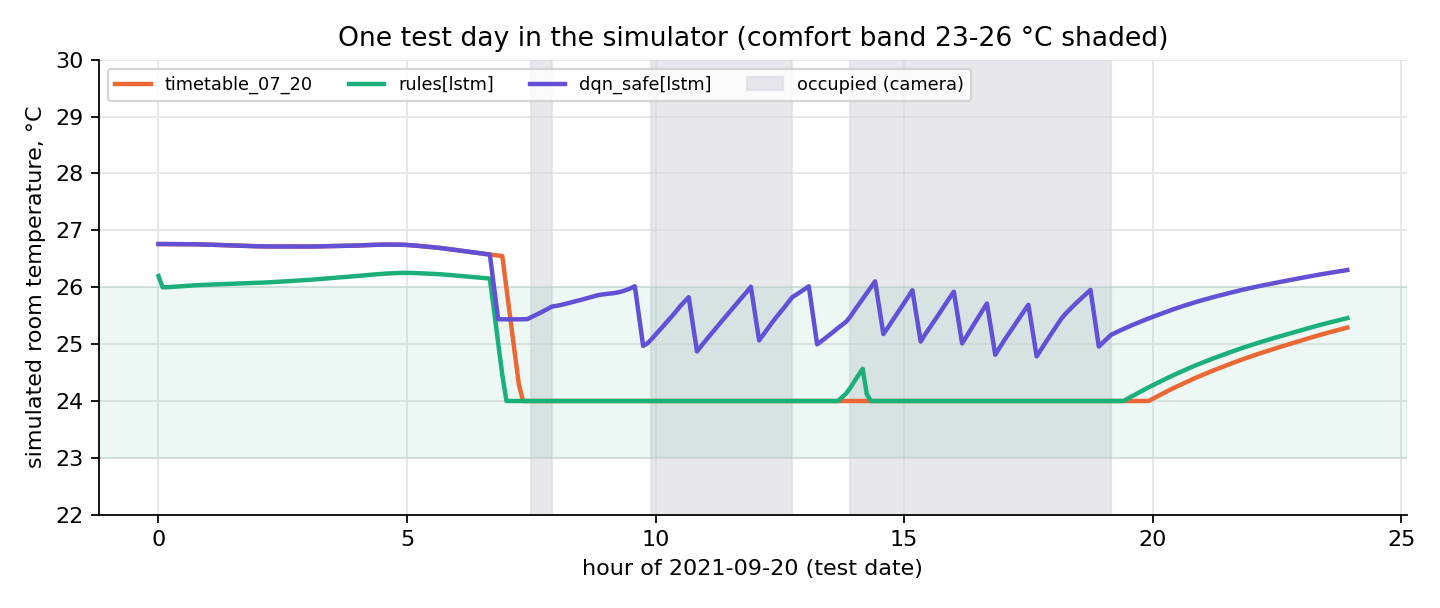
\includegraphics[width=0.85\textwidth]{closed_loop_day.png}
\caption{One simulated test day: room temperature under each controller}
\label{fig:day}
\end{figure}

\section{Performance Evaluation}
\textbf{Live run} (one machine, through its network interface):
\begin{itemize}
\item 290 readings (288 replay + 2 demonstration messages), 290 decisions, 6 $\times$ 290 predictions;
\item 29 commands, 100\% acknowledged;
\item round trip: median 88~ms, p95 92~ms, max 93~ms;
\item telemetry-to-actuator loop: median 94~ms, p95 159~ms;
\item per-model inference 1.0--12.7~ms, and 38--54~ms for all six models per reading.
\end{itemize}

\begin{figure}[H]
\centering
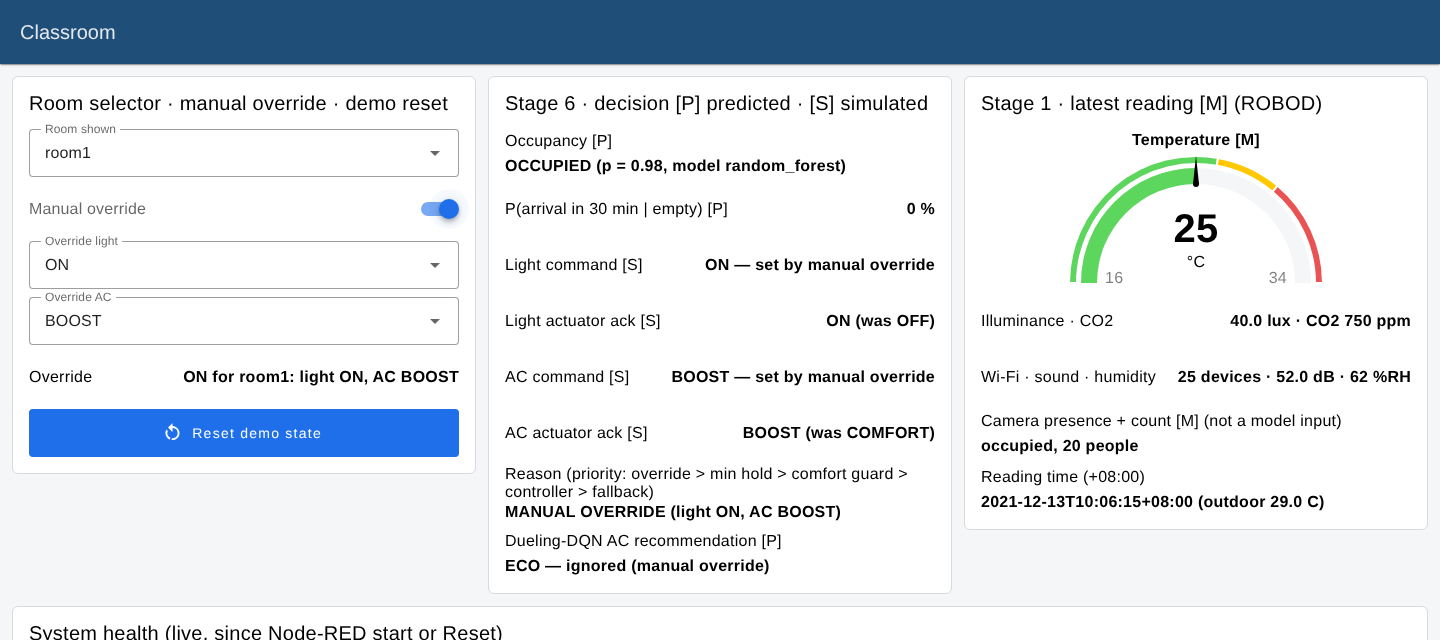
\includegraphics[width=0.9\textwidth]{manual_override.png}
\caption{Manual override applied, sent over MQTT and acknowledged in 87~ms}
\label{fig:override}
\end{figure}

\section{Testing}
The command \texttt{python -m pytest -q} gives \textbf{97 passed, 1 skipped} (the skip is the opt-in end-to-end
test). The end-to-end test, run separately, also passes: real broker, Node-RED, ML service, actuator and replay, with
100\% of commands acknowledged. A clean-room run from the delivered ZIP, with a fresh official dataset download, gave
the same results.

\begin{table}[H]
\centering
\caption{Automated tests by area}
\label{tab:tests}
\small
\begin{tabularx}{\textwidth}{@{}L{3.6cm}cY@{}}
\toprule
\textbf{Test file} & \textbf{Tests} & \textbf{Covers}\\
\midrule
test\_data\_features & 9 & schema, units, timestamps, no silent filling, date splits, no future information, live = offline features\\
test\_models\_eval & 7 & every category trains and predicts, save/load, seeded training, dueling head, report consistency, fallback\\
test\_messages\_actuator & 4 & strict JSON telemetry, actuator accepts/rejects, separate devices\\
test\_flow\_functions & 19 & validation, duplicates, stale data, gate ids, ACK, savings and comfort counters, SQLite-driven panels\\
test\_rules & 14 & hysteresis, grace, AC off, BOOST, pre-cool, hold, start-up, override, DQN + safety, displayed decision source\\
test\_config\_flows & 13 & flow wiring, schema = flow, no secrets in flows, pinned packages, broker ACL\\
test\_failures & 19 & broker down/restart, wrong credentials, ACL, ML crash, missing model, DB locked, late/unknown ACK, dataset tampering\\
test\_scripts & 12 & setup/start/stop scripts, shell and PowerShell parsing, firewall scope\\
test\_e2e\_loopback (opt-in) & 1 & full system with 60 readings\\
\bottomrule
\end{tabularx}
\end{table}

Testing found and fixed four real defects:
\begin{itemize}
\item duplicate command ids within one millisecond;
\item late acknowledgements after the timeout being ignored;
\item a stop script returning before Node-RED had exited;
\item an editor session file tracked by version control.
\end{itemize}

\section{Two-Laptop Deployment}
Laptop~1 runs \texttt{setup\_server.ps1}, then \texttt{open\_firewall.ps1} (once, as Administrator), then
\texttt{start\_server.ps1}. Laptop~2 runs \texttt{setup\_node.ps1 -ServerIp <IP>}, then \texttt{start\_node.ps1}.
Shutdown uses \texttt{stop\_node.ps1} and \texttt{stop\_server.ps1}.

The scripts:
\begin{itemize}
\item detect Python, Node.js and Mosquitto, and install the dependencies;
\item generate random credentials and validate the environment and the dataset hash;
\item refuse to start on a busy port, naming the owning process;
\item print the LAN IP, test TCP and MQTT login from the node, and record process ids for clean shutdown.
\end{itemize}

\textbf{Verification status.} The PowerShell scripts pass the real PowerShell parser, and the Linux equivalents ran
the complete system. Operation on two separate physical laptops is prepared, with a 15-item checklist, but had not
been verified at the time of writing.

% ---------------------------------------------------------------- Chapter 6
\chapter{Conclusion and Future Work}\label{ch:concl}

\section{Conclusion}
The system implements all eight reference stages: authenticated MQTT, Node-RED integration, SQLite, a Node-RED
dashboard that reads its evaluation results from the database, and a complete command and acknowledgement loop.
Delivery is measured: 100\% of commands were acknowledged, with a round trip of about 0.09~s.

Traditional, ensemble and deep models, including the two research adaptations, were compared on held-out dates
without test-set selection. Mamba scored highest on test, but the differences are within the date-to-date
uncertainty, and the validation-selected random forest remains the primary model.

Occupancy-driven rules halved simulated cooling energy at under 1\% comfort violations. The paper-B Dueling DQN saves
more energy but needs a stronger comfort weight, so it stays optional behind a safety layer.

Every number in this report is traceable to a result file, and every saving is a simulation result.

\section{Limitations}
\begin{enumerate}
\item \textbf{Small data:} 29 dates, of which 6 are test dates (two nearly empty), so model rankings are not
  statistically separable.
\item \textbf{OCC-Mamba} is followed only at the model-family level.
\item \textbf{Grey-box plant} with assumed parameters: absolute closed-loop energy is indicative only.
\item \textbf{Counterfactual energy} assumes energy scales with our command, so savings are optimistic.
\item \textbf{Lighting comfort:} lights are wrongly OFF in 8--28\% of occupied intervals, depending on room and split.
\item \textbf{DQN:} the comfort weight is too low and switching is frequent.
\item \textbf{Security:} no TLS on MQTT, and the dashboard controls have no login on the LAN.
\item \textbf{Not verified:} two physical laptops, physical actuators and the dataset licence.
\end{enumerate}

\section{Future Work}
\begin{itemize}
\item Add a PIR motion sensor or a minimum-lighting fallback to remove wrong lights-OFF.
\item Tune the DQN reward (comfort weight, switching penalty, previous action in the state) on validation dates.
\item Use more dates and rooms for stable model selection, and report confidence intervals as standard.
\item Add TLS for MQTT and a login for the dashboard controls.
\item Obtain the OCC-Mamba full text to align the architecture.
\item Run a pilot in a real room with relays and metered energy.
\end{itemize}

\section{Team Contributions}
The decision engine, Dueling DQN and energy evaluation is the largest machine-learning part of the project, and was
shared by two members.

\begin{table}[H]
\centering
\caption{Team members and subsystems}
\label{tab:team}
\small
\begin{tabularx}{\textwidth}{@{}L{4.6cm}L{3.7cm}Y@{}}
\toprule
\textbf{Member} & \textbf{Roll Number} & \textbf{Subsystem}\\
\midrule
NIRANJAN N S & AM.SC.U4CSE23338 & decision engine, Dueling DQN, energy and comfort evaluation (shared with Sivadev Smijith)\\
SIVADEV SMIJITH & AM.SC.U4CSE23359 & decision engine, Dueling DQN, energy and comfort evaluation (shared with Niranjan N S); Node-RED integration, SQLite, dashboard\\
YALAMARTHI JYOTHI SRI KRISHNA CHAITANYA & AM.SC.U4CSE23370 & IoT node, MQTT broker, security, two-laptop deployment\\
PENUMALLU RAM DINESH REDDY & AM.SC.U4CSE23341 & dataset, features, traditional and ensemble ML, evaluation\\
MANISH SHISHIRCHANDRA DORA ALURI & AM.SC.U4CSE23333 & LSTM and Mamba models, ML service\\
\bottomrule
\end{tabularx}
\end{table}

% ---------------------------------------------------------------- References
\chapter*{References}
\addcontentsline{toc}{chapter}{References}
\markboth{REFERENCES}{}
\begin{enumerate}[label={[\arabic*]},leftmargin=*]
\item Z.~D. Tekler, Y.~Lei, Y.~Peng, C.~Miller and A.~Chong, ``ROBOD, room-level occupancy and building operation
  dataset,'' \emph{Building Simulation}, vol.~15, no.~12, 2022. doi:10.1007/s12273-022-0925-9. Data:
  https://github.com/ideas-lab-nus/robod
\item I.~Qaisar, K.~Sun, D.~Zhong, X.~Yang, X.~Miao and Q.~Zhao, ``OCC-Mamba: A Mamba-based deep learning approach
  for indoor occupancy prediction,'' \emph{Building and Environment}, article 114085, 2025.
  doi:10.1016/j.buildenv.2025.114085 (record verified; full text not accessed).
\item F.~Hou, J.~C.~P. Cheng, J.~Ma, H.~H.~L. Kwok, C.~Huang and Z.~Wu, ``Occupancy-driven HVAC control optimization
  via LSTM and deep reinforcement learning for enhanced indoor air quality, thermal comfort and energy efficiency,''
  \emph{Building and Environment}, vol.~284, 113501, 2025. doi:10.1016/j.buildenv.2025.113501
\item A.~Gu and T.~Dao, ``Mamba: Linear-time sequence modeling with selective state spaces,'' arXiv:2312.00752, 2023.
\item Z.~Wang, T.~Schaul, M.~Hessel, H.~van Hasselt, M.~Lanctot and N.~de Freitas, ``Dueling network architectures for
  deep reinforcement learning,'' in \emph{Proc. ICML}, 2016. arXiv:1511.06581
\item K.~Sun, I.~Qaisar, M.~A. Khan, T.~Xing and Q.~Zhao, ``Building occupancy number prediction: A Transformer
  approach,'' \emph{Building and Environment}, vol.~244, 110807, 2023.
\item OASIS, \emph{MQTT Version 3.1.1}, OASIS Standard, 2014.
\item Eclipse Foundation, \emph{Eclipse Mosquitto documentation} (mosquitto.conf, password file and ACL).
\item OpenJS Foundation, \emph{Node-RED 4 documentation}; FlowFuse, \emph{Node-RED Dashboard 2.0 documentation}.
\end{enumerate}

% ---------------------------------------------------------------- Appendix
\appendix
\chapter{Reproduction Instructions}
{\footnotesize
\begin{verbatim}
# Laptop 1 (Linux/macOS; Windows: the .ps1 equivalents)
bash scripts/setup_server.sh          # venv, deps, .env with random passwords,
                                      # dataset + SHA-256, models, npm, broker users, DB
python download_data.py --verify      # PASS x2: sha256 matches, 8352 rows, schema ok
python train_models.py                # ~10 min CPU; models/ and results/ (seed 42)
python run_experiments.py             # counterfactual + closed loop; results/*.csv
python tools/bootstrap_ci.py          # supplementary confidence intervals
python -m pytest -q                   # 97 passed, 1 skipped
SC_E2E=1 python -m pytest -q tests/test_e2e_loopback.py   # 1 passed
bash scripts/start_server.sh          # then on Laptop 2:
bash scripts/start_node.sh --date 2021-09-20
\end{verbatim}
}

\textbf{Versions and configuration:}
\begin{itemize}
\item Python 3.13.17, Node.js 22.23.4, Mosquitto 2.0.18, node-red 4.1.17; Python packages pinned in
  \texttt{requirements*.txt}.
\item Seeds 42 throughout.
\item Splits and features are recorded in \texttt{models/training\_report.json}; the model manifest is in
  \texttt{models/final/manifest.json}.
\item Thresholds are in the Node-RED CONFIG node; simulator parameters are in \texttt{smartclass/room\_env.py}.
\end{itemize}

\end{document}
